\chapter{Full Posit Processing Unit (PPU)}

In this Chapter we extend the architecture seen in Section 6.5, adding the capability for arithmetic operations between posits - that is, addition, subtraction, multiplication and division.



\section{Single-stage Architecture}

In the following Sections we refer to a PPU design with a single-stage of computation. This means that the unit is a single combinatory logic component from input to output.

Theoretically, this means that:
\begin{itemize}
    \item We are sure that, in 1 clock cycle, the component will output its result
    \item The end-to-end latency can negatively affect the drive clock fed to the unit. Indeed, if we imagine the unit being integrated into a more complex system (e.g. a full processor), its inputs and outputs will be fed from/into registers. In order to respect timing constraints of registers the clock period must be adjusted to the the latency of the processor components. If the PPU unit is has a sufficiently large end-to-end latency, this can impact the clock frequency for the whole processor, slowing down the whole system.
\end{itemize}

From a high-level standpoint the main building blocks are the ones highlighted in Figure \ref{fig:overview_ppu}.
The operands are converted into the agnostic FIR datatype via the \textit{extraction} stage; the \textit{computation} stage is in charge of implementing addition, subtraction, multiplication, and division according the control signal that determines the operation; lastly the \textit{normalization} stage implements all the steps necessary to convert back the agnostic output from the operation into a posit bit-string.

\begin{figure}
    \begin{center}
    \includegraphics[width=0.9\textwidth]{figures/top.pdf}
    \caption{Single stage configuration for a PPU unit}
    \label{fig:overview_ppu}
    \end{center}
\end{figure}

\section{Datapath}

\subsection{Extraction}\label{sec:posit_extraction}

The extraction module (Figure \ref{fig:extraction_ppu}) performs a preliminary input conditioning (Figure \ref{fig:input_conditioning_module} on the posit inputs, followed by the actual field extraction.

The input conditioning is used to 
\begin{itemize}
    \item perform simple operands swapping if either the second operand encode a negative value, or the second operand encodes a larger (absolute) value than the first 
    \item detect special and trivial cases, depending on the operation considered (e.g. we have a sum and one of the two inputs is zero).
\end{itemize} 

If the latter occurs, \texttt{special} if forwarded straight to the output of the PPU and delivers the result to the outer world. These cases are resolved at posit bit-string level (i.e. pre-decoding) and don't involve the remaining two intermediate stages.

\begin{figure}
    \centering
    \includegraphics[width=0.87\textwidth]{figures/extraction.drawio.pdf}
    \caption{Extraction module}
    \label{fig:extraction_ppu}
\end{figure}

\begin{figure}
    \centering
    \includegraphics[width=0.9\textwidth]{figures/posit2fir.drawio.pdf}
    \caption{Posit to FIR module}
    \label{fig:posit2fir_ppu}
\end{figure}






\begin{figure}
    \centering
    \includegraphics[width=.75\textwidth]{figures/input_conditioning.pdf}
    \caption{Input conditioning module}
    \label{fig:input_conditioning_module}
\end{figure}



\textit{Posit to FIR} (Figure \ref{fig:posit2fir_ppu}) takes a \texttt{N}-bit bitstring encoding a posit and outputs a \texttt{FIR\_SIZE}-bit\footnote{\texttt{1 + TE\_SIZE + FRAC\_SIZE} = \texttt{1 + [(ES + 1) + (clog2(N) + 1)] + (N - 2)}} bistring encoding the concatenation of \textit{sign}, the total exponent \textit{te}, and the fraction \textit{frac}.
The heavy lifting of the operation is done by \textit{posit unpack} which extracts and decodes the fields off the posit. The principle is not dissimilar from the extraction of binary32 fields, but the implementation is more complex , since the size of the regime is not static and additional decoding steps are needed to compute its length.
The core piece of hardware in charge of decoding the regime is presented by the leading-zero counter (LZC). The idea behind the LZC is an iterative approach. There exist different implementations for the LZC and we will cover the main ones hereafter.

\paragraph{Naive LZC}

A naive version of a LZC can be implemented using an hardware loop that checks for adjacent zeros. While the behavior is correct, the cost of this implementation is nontrivial: let's consider the RTL schematic in Figure \ref{fig:lzc_sinthesyzed}.



%%%%% make figure larger than main margins: https://tex.stackexchange.com/a/57706/271788
\begin{figure}[h!]
    \noindent\makebox[\textwidth]{%
        \includegraphics[width=1.3\textwidth]{figures/lzc_naive_quartus.pdf}}
    \caption{Naive 16-bits LZC generated schematic}
    \label{fig:lzc_sinthesyzed}
\end{figure}



Notice that this is a long chain of multiplexers and equal tests, that grows proportionally -- $\mathcal{O}(n)$ -- to the number of input bits. While this would work, the longest signal propagation path would grow out of hand, making this component unsuitable to be used at a very high speed.

\paragraph{Tree-based LZC}

A tree-based solution would bring the benefit of reducing the longest chain from $\mathcal{O}(n)$ to $\mathcal{O}(\log(n))$ which, in turn, would increase the highest achievable speed the circuit could safely run at.


The design devised by \cite{milenkovic_modular_2015} proposes a so-called modified-tree structure. The computation is divided in group of 4 bits which are fed into a 8-bits unit, and eventually \textit{mux}-ed out.
The downside of this design is that it requires the input to have a number of bits which is a power of $2$ in order to justify its adoption.

\begin{figure}
        \centering
        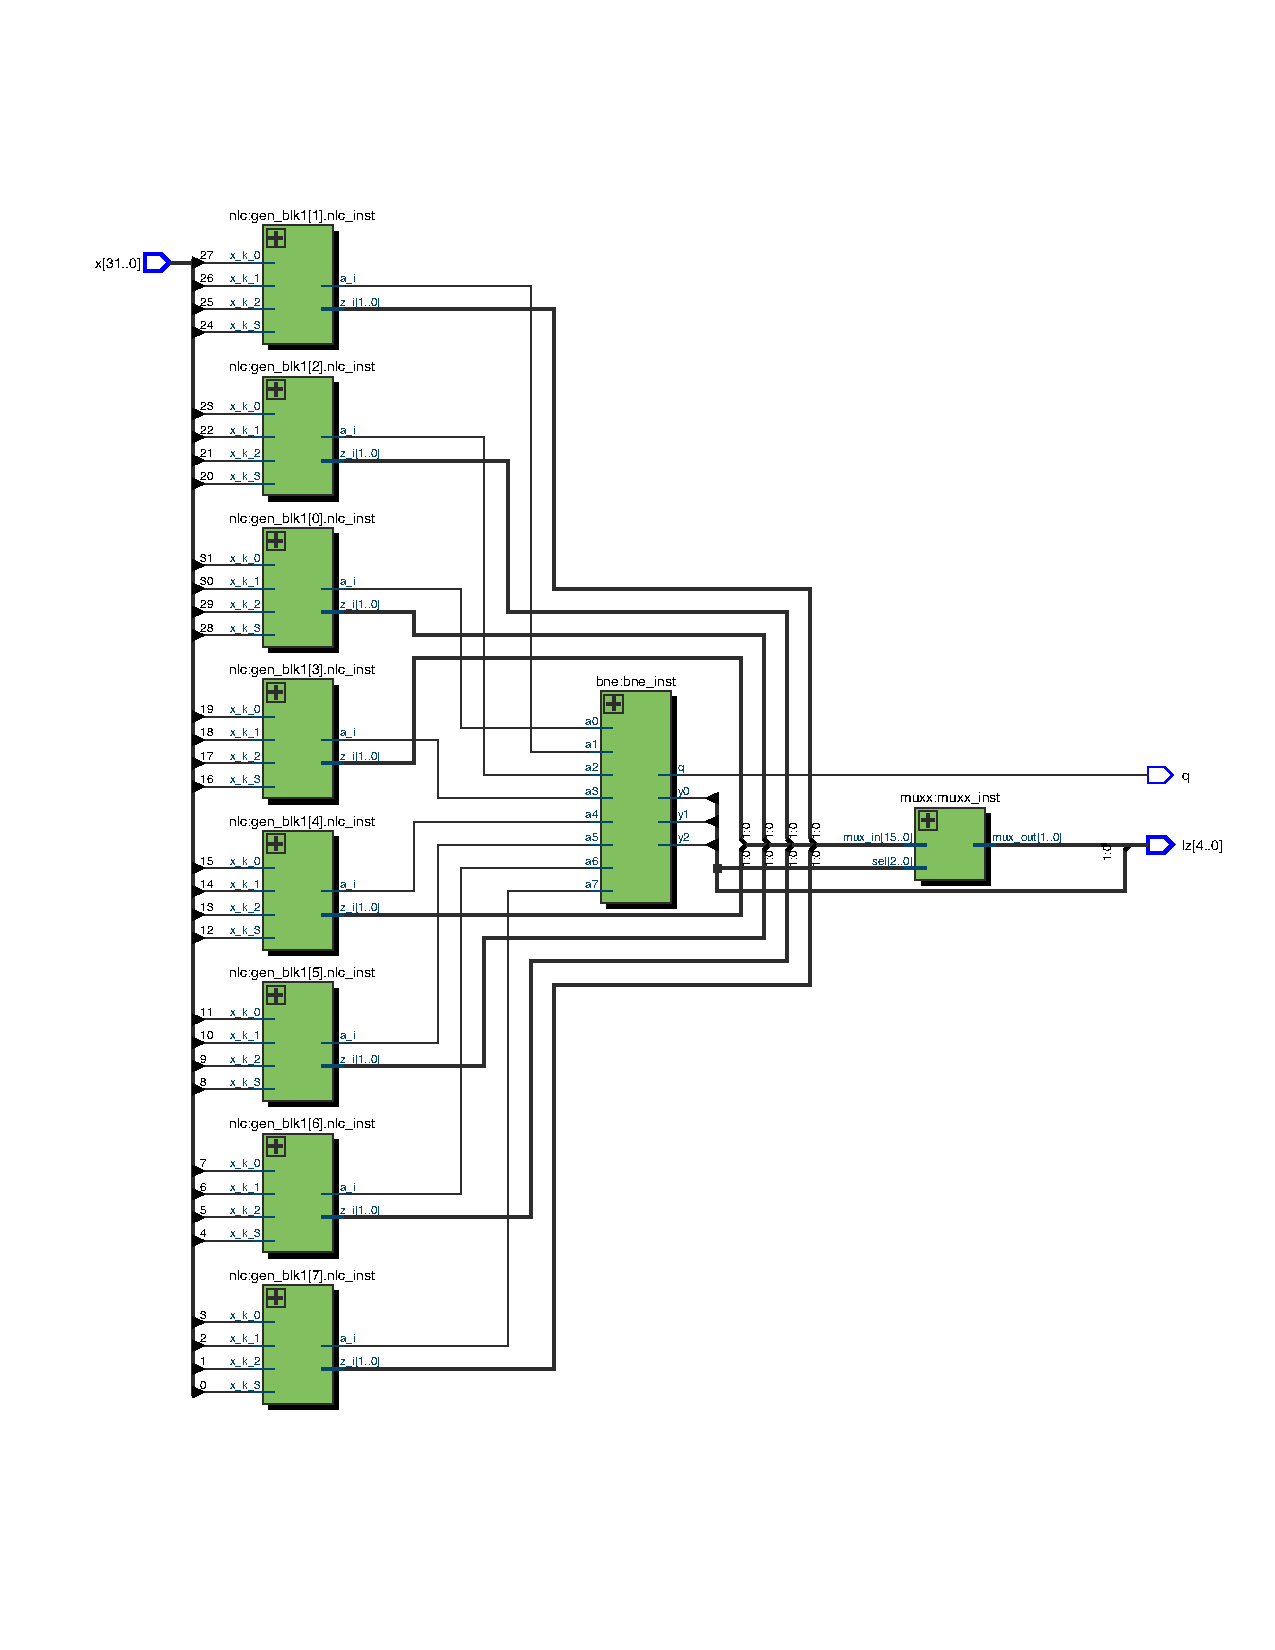
\includegraphics[width=\textwidth]{figures/milenkovic_quartus1.pdf}
\end{figure}

\begin{figure}
    \centering
    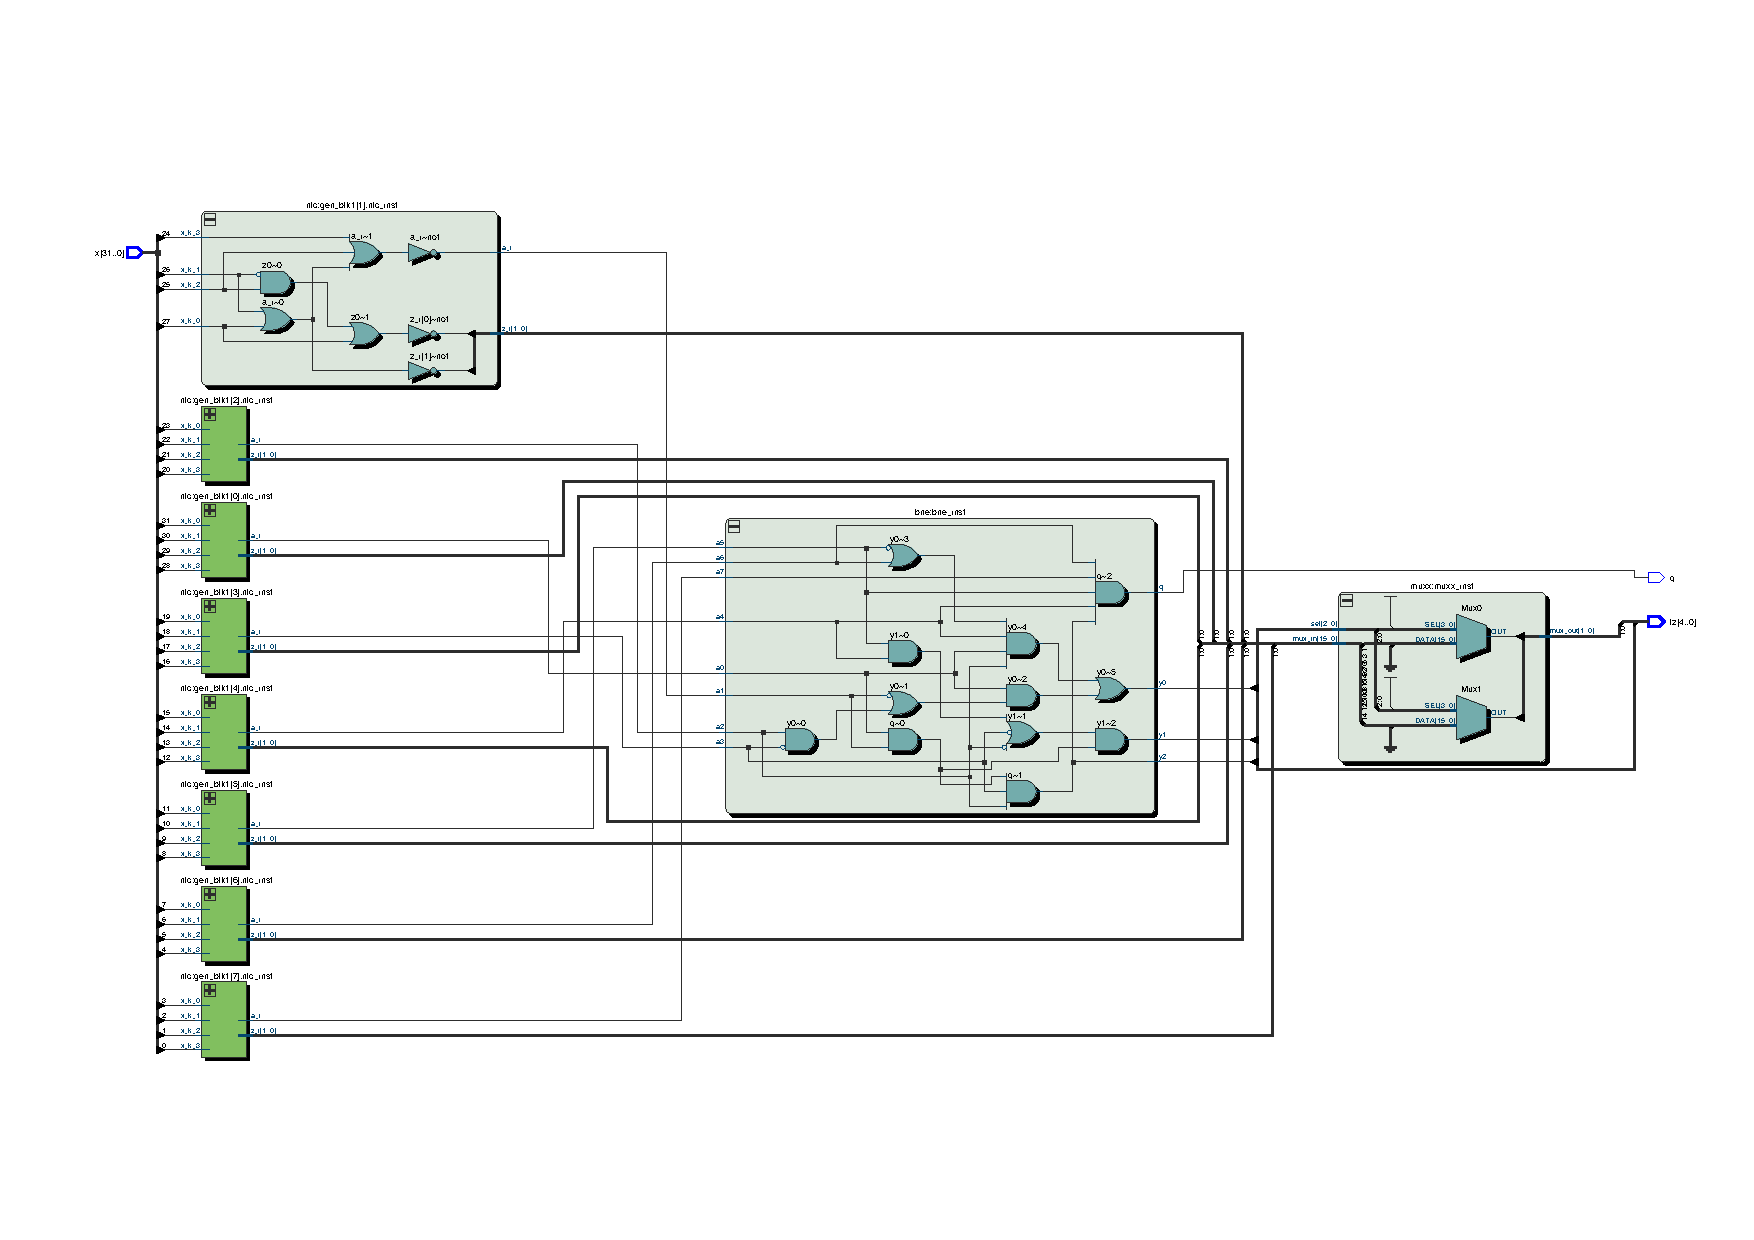
\includegraphics[width=\textwidth]{figures/milenkovic_quartus2.pdf}
    \caption{\cite{milenkovic_modular_2015}'s 16-bits LZC generated schematic}
    \label{fig:milenkovic_lzc_quartus}
\end{figure}


A similar design is presented by \cite{dimitrakopoulos_low-power_2008}, which proposes a semi-tree based approach acting on 16 bits at a time. Like the previous design, this can be extended to other larger power of $2$ input bits configurations.

\paragraph{Pacogen LZC}

Yet another design was proposed by \cite{PACoGen}.
Here, same basic building block is recursively instantiated, terminating in a simple \textit{and} / \textit{or} gates pair, which make up the base case (figure \ref{fig:pacogen_LOD2_1}).
The truth table (\ref{table:lod21_truth_table}) of \ref{fig:pacogen_LOD2_1} indicates that, at the lowest level, $k$ counts the number of zeros from the left. A sequence without bit alternation is considered invalid, as the $\text{vld}$ flags reports.

The higher-level hierarchical block (4:2) is shown in figure \ref{fig:lod42_00001} and consists of two instances of \ref{fig:pacogen_LOD2_1} together with a \textit{or} gate and a multiplexer that routes out the correct $k$ from the ``child" instance, left-wise padded with either a $0$ or $1$.

The truth table gives an idea about how \ref{table:lod21_truth_table} extends onwards.
\begin{table}[h!]
\centering
    \begin{minipage}{0.5\linewidth}
        \centering
        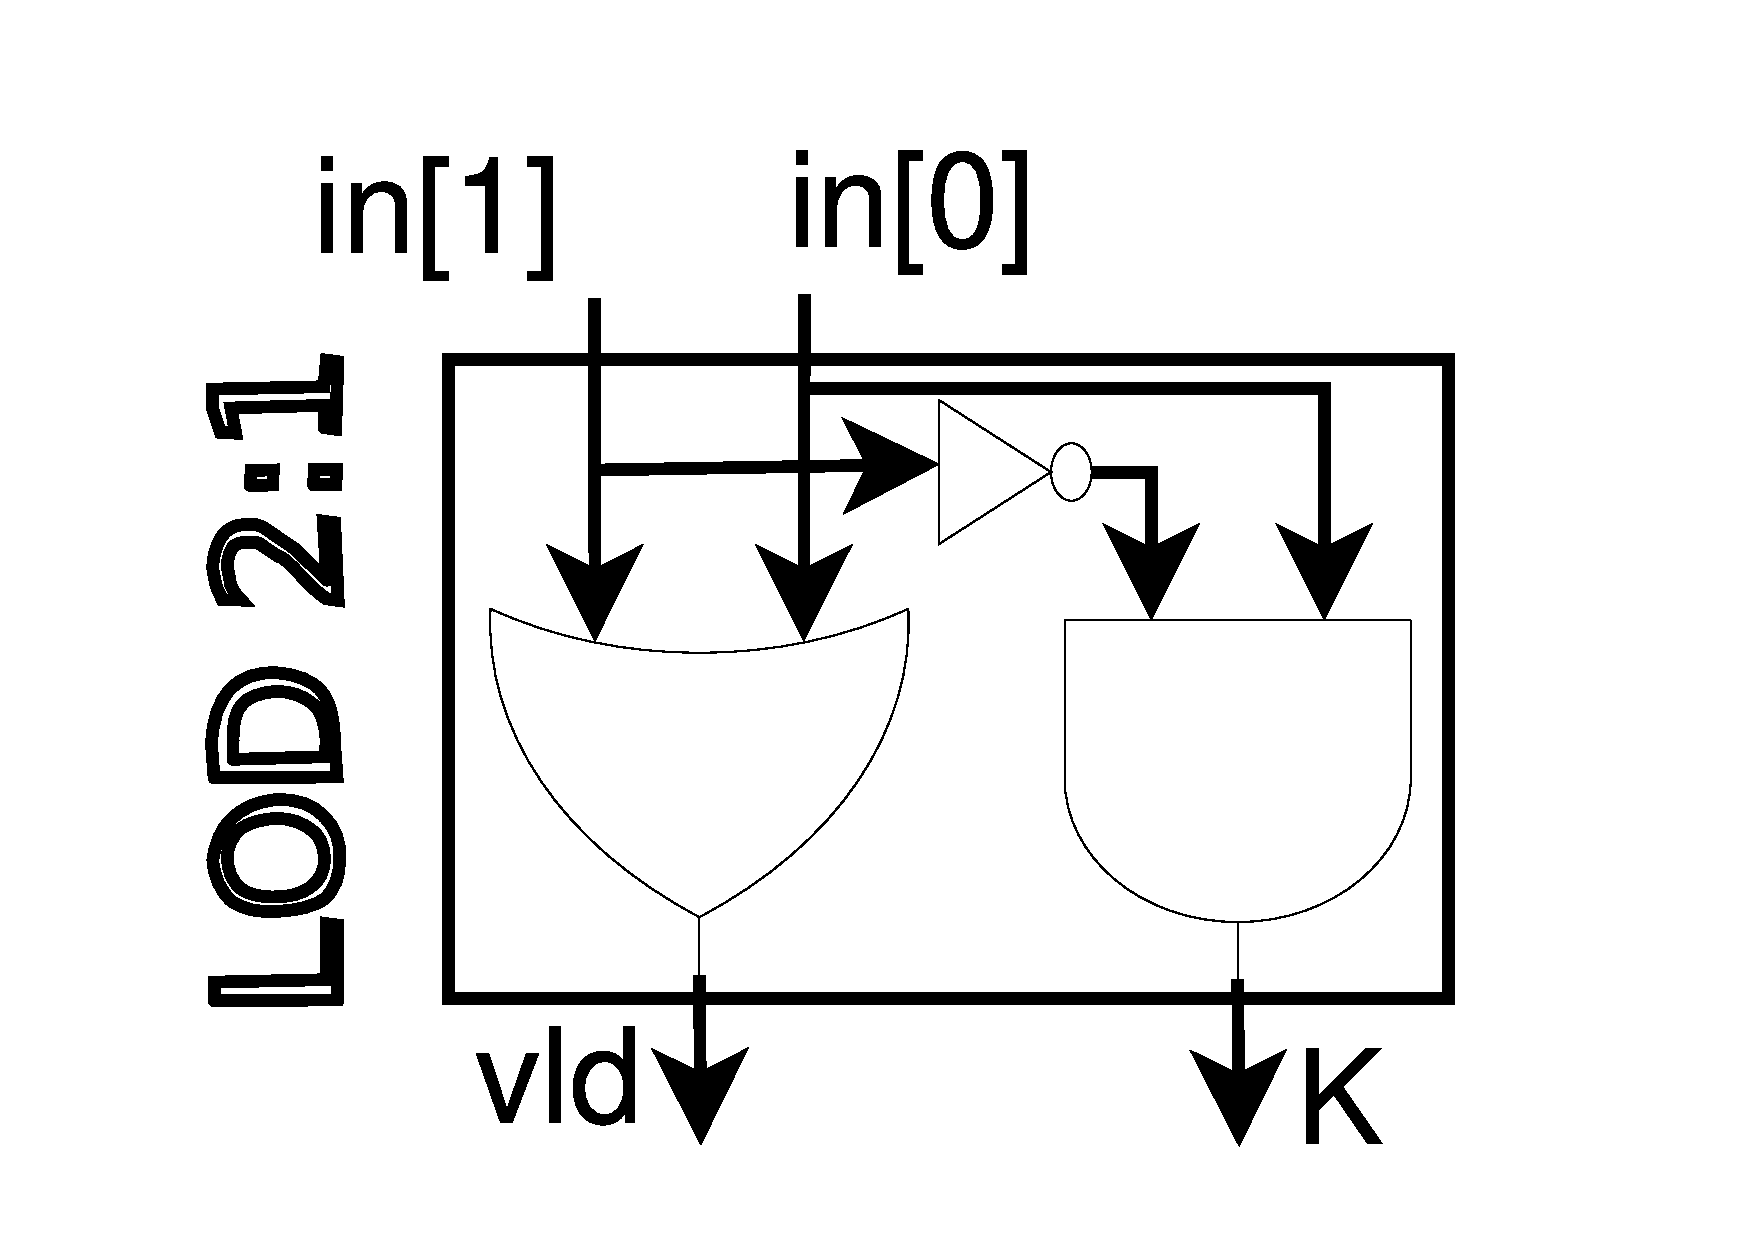
\includegraphics[
            %scale=1
            width=0.85\linewidth]{figures/lod2_1.pdf}
        \captionof{figure}{\cite{PACoGen}'s LOD 2:1 block}
        \label{fig:pacogen_LOD2_1}
    \end{minipage}\hfill
    \begin{minipage}{0.5\linewidth}
        \centering
        \begin{tabular}{cccc}
            \toprule
            \multicolumn{2}{c}{in} & vld & k \\
            \cmidrule{1-2} %\cmidrule{3-3} \cmidrule{4-4}
            0 & 0 & \textbf{0} & 0 \\
            0 & 1 & 1 & 1 \\
            1 & 0 & 1 & 0 \\
            1 & 1 & 1 & 0 \\
            \bottomrule
        \end{tabular}
        \captionof{table}{LOD 2:1 truth table}
        \label{table:lod21_truth_table}
    \end{minipage}
\end{table}

\begin{figure}[h!]
    \begin{minipage}[b]{0.5\linewidth}
        \iffalse
        \centering
        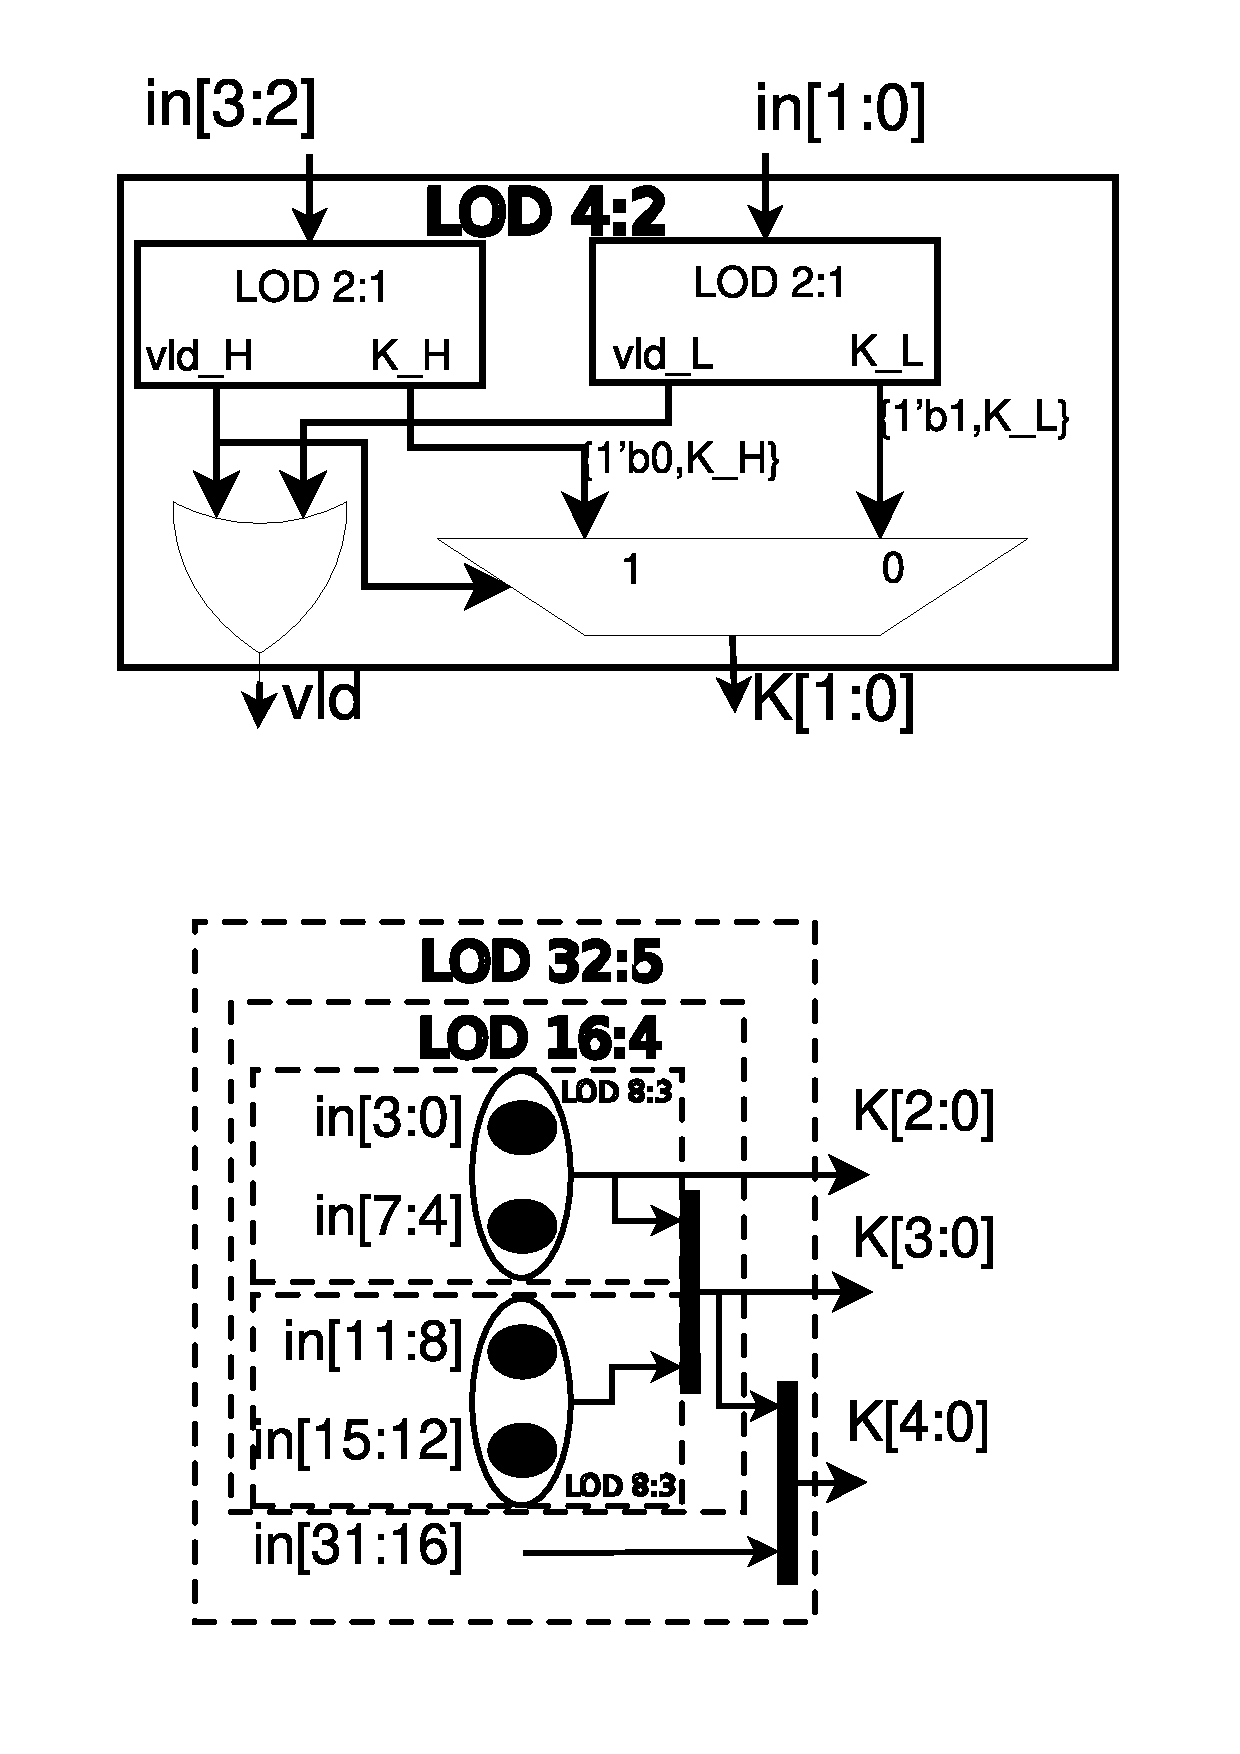
\includegraphics[
            %scale=1
            width=0.8\linewidth,
            valign=t]{figures/pacogen_LODS.pdf}
        \captionof{figure}{\cite{PACoGen}'s LZC architectural building blocks}
        \label{fig:pacogen_LOD_arch}
        \fi

        \centering
        \begin{minipage}{0.6\textwidth}
            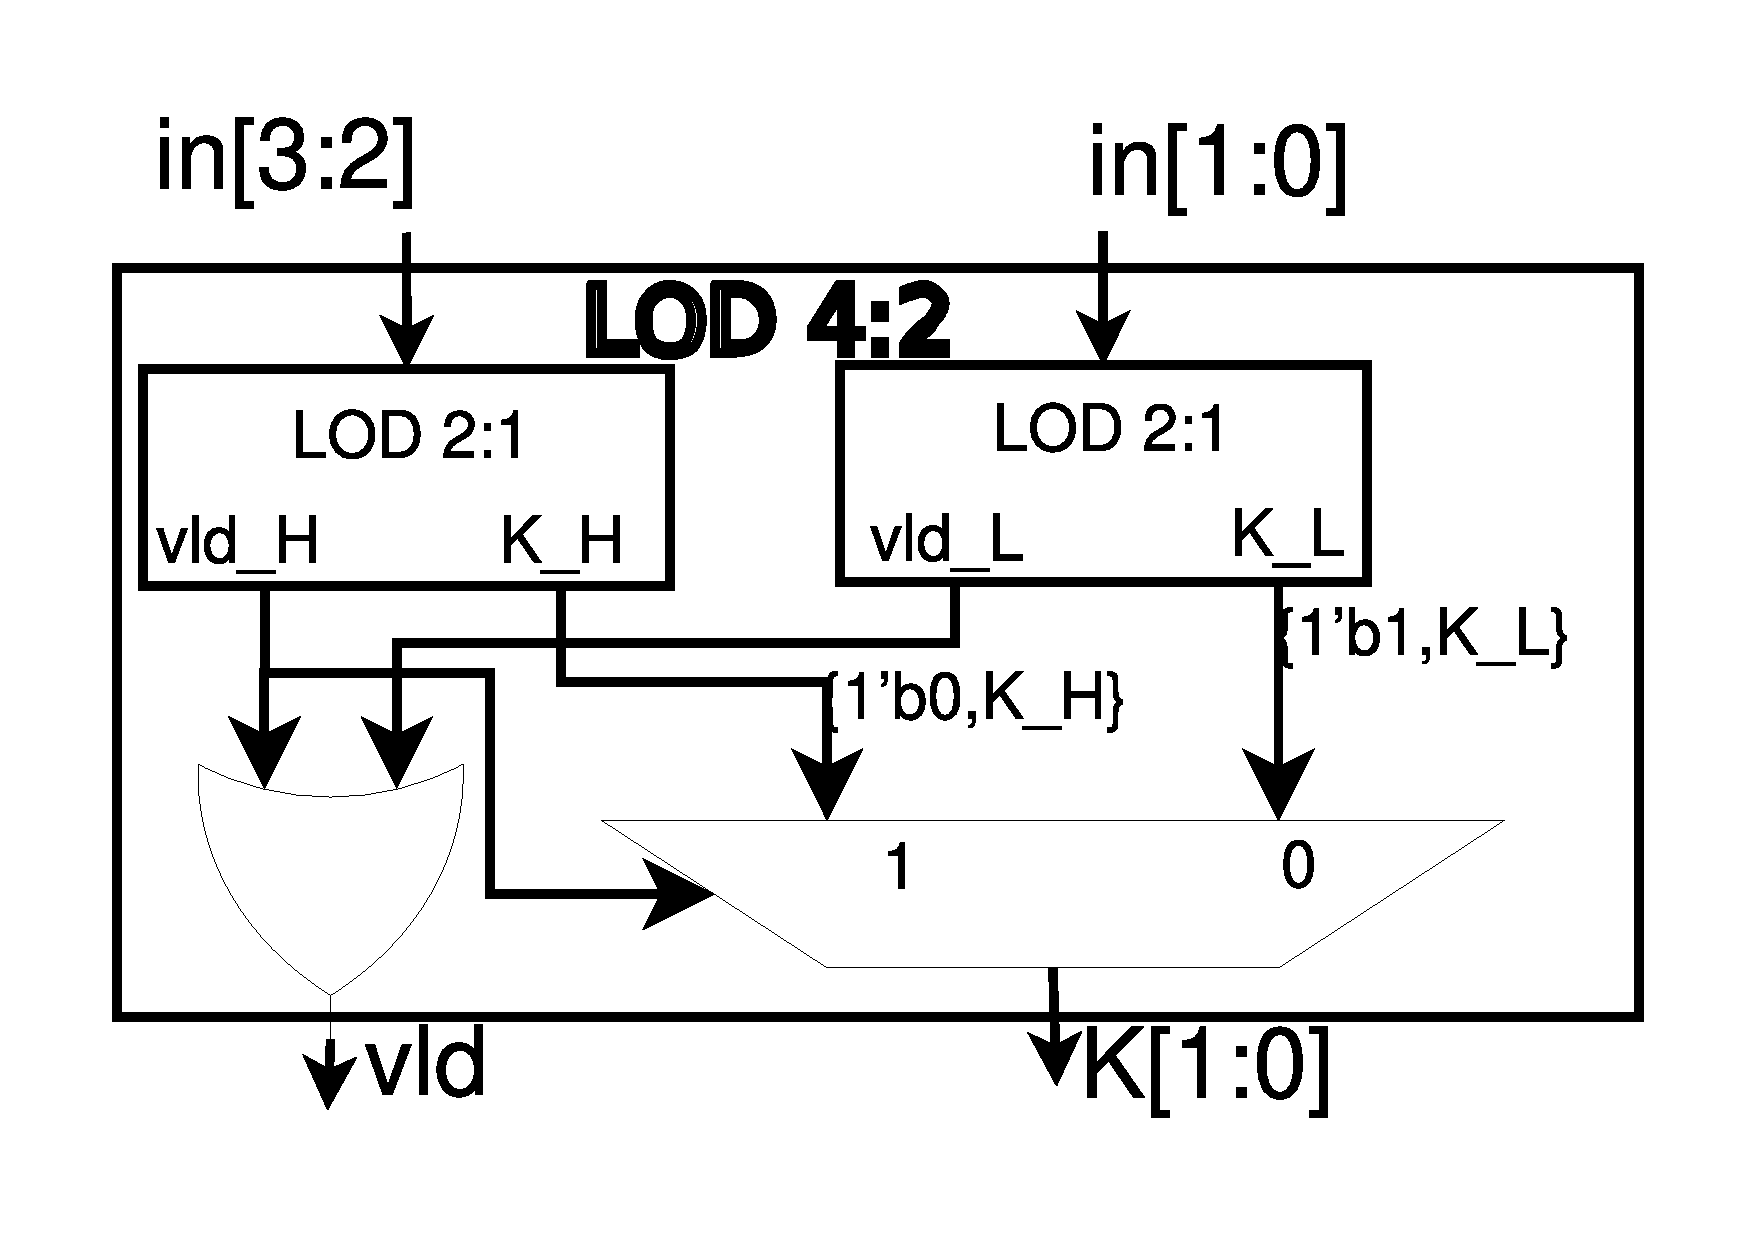
\includegraphics[width=\textwidth]{figures/lod4_2.pdf}
            \caption{LOD 4:2 block}
            \label{fig:lod42_00001}
        \end{minipage}
        \vfill
        \begin{minipage}{0.6\textwidth}
            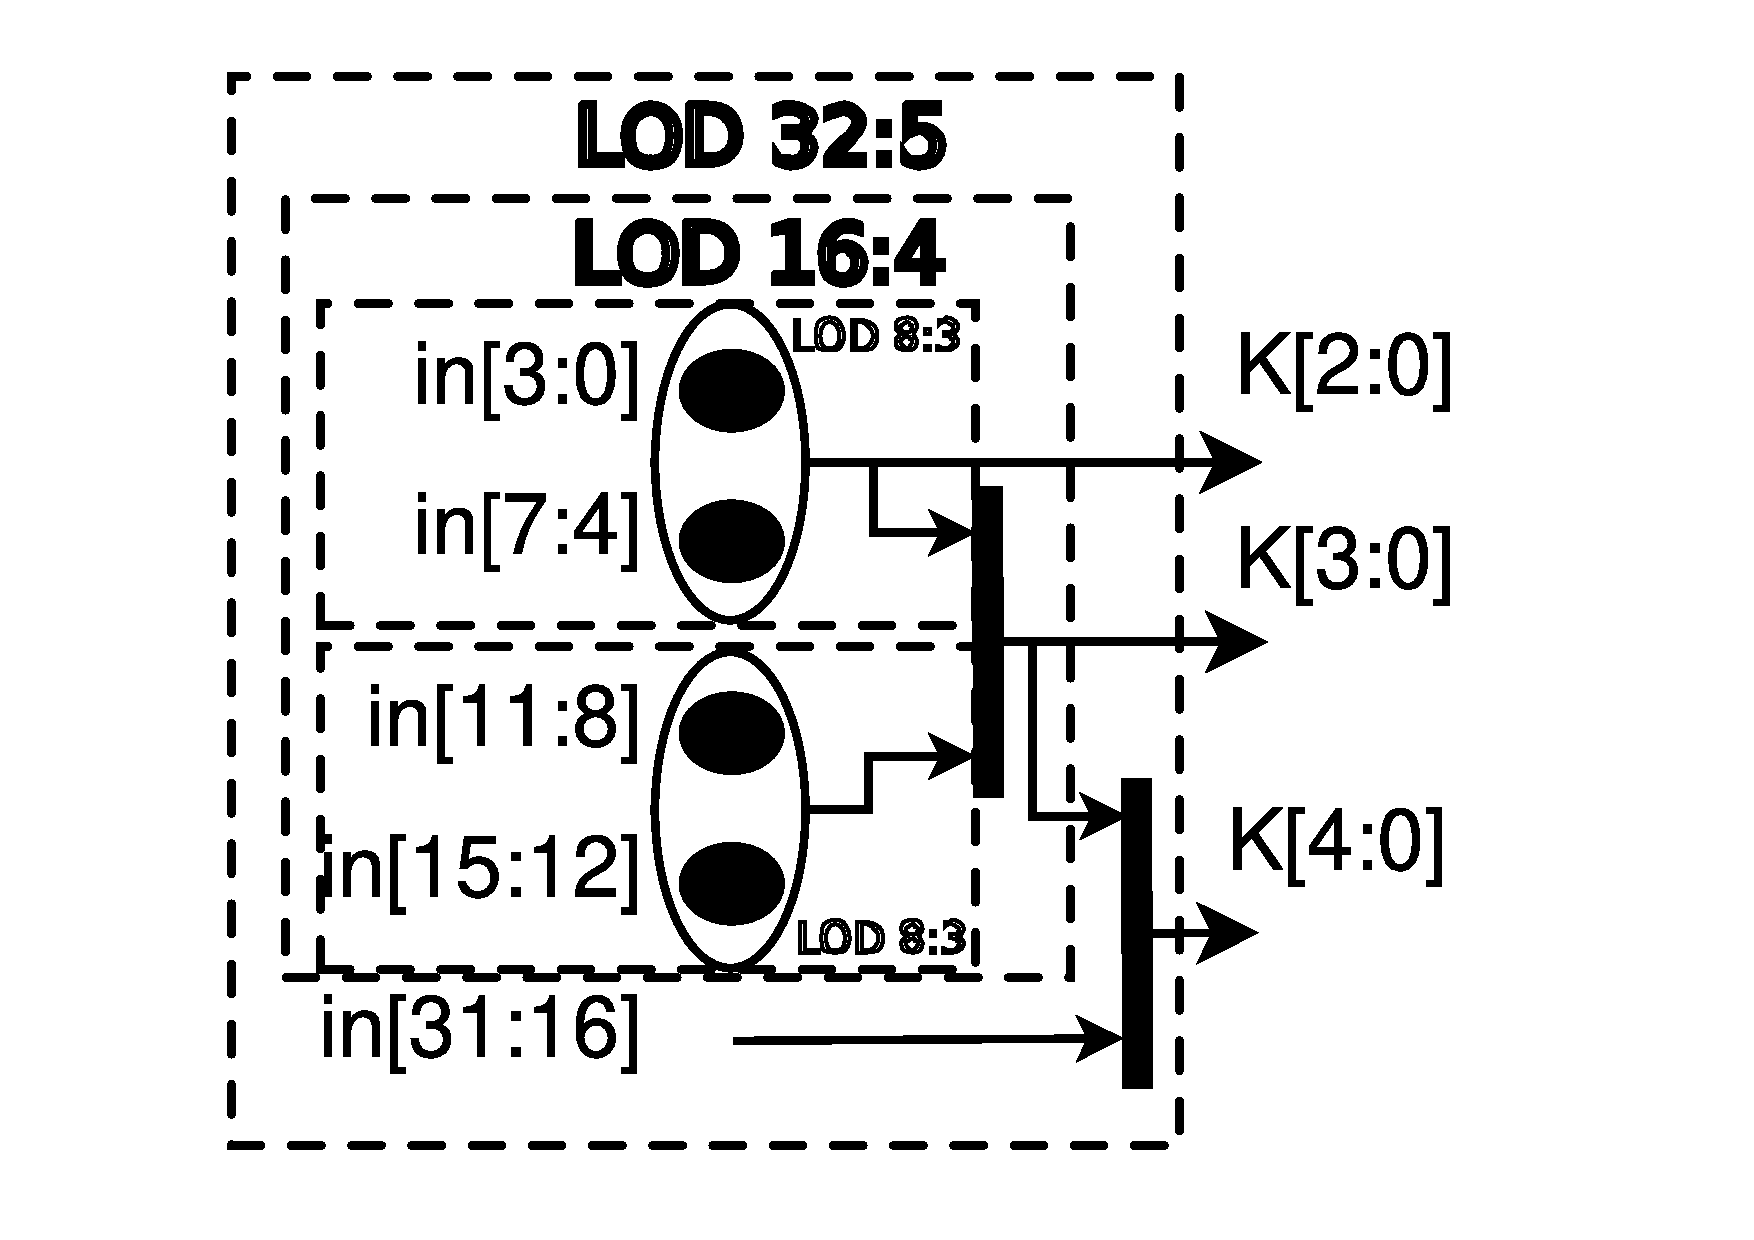
\includegraphics[width=\textwidth]{figures/lod32_5.pdf}
            \caption{LOD 32:5 block}
            \label{fig:lod16_4_0000}
        \end{minipage}
        \captionof{figure}{\cite{PACoGen}'s LZC architectural building blocks}
        \label{fig:pacogen_LOD_arch}
    \end{minipage}
    %
    \begin{minipage}[b]{0.5\linewidth}
        \centering
        \begin{tabular}{cccccccccc}
        \toprule
        \multicolumn{4}{c}{in} & $\text{vld}_l$ & $\text{vld}_h$ & vld & $\text{k}_l$ & $\text{k}_h$ & k \\
        \cmidrule{1-4} %\cmidrule{5-5} \cmidrule{6-6} \cmidrule{7-7} \cmidrule{8-8} \cmidrule{9-9}
        0 & 0 & 0 & 0 & 0 & 0 & \textbf{0} & 0 & 0 & 10 \\
        0 & 0 & 0 & 1 & 1 & 0 & 1 & 0 & 1 & 11 \\
        0 & 0 & 1 & 0 & 1 & 0 & 1 & 0 & 0 & 10 \\
        0 & 0 & 1 & 1 & 1 & 0 & 1 & 0 & 0 & 10 \\
        0 & 1 & 0 & 0 & 0 & 1 & 1 & 1 & 0 & 01 \\
        0 & 1 & 0 & 1 & 1 & 1 & 1 & 1 & 1 & 01 \\
        0 & 1 & 1 & 0 & 1 & 1 & 1 & 1 & 0 & 01 \\
        0 & 1 & 1 & 1 & 1 & 1 & 1 & 1 & 0 & 01 \\
        1 & 0 & 0 & 0 & 0 & 1 & 1 & 0 & 0 & 00 \\
        1 & 0 & 0 & 1 & 1 & 1 & 1 & 0 & 1 & 00 \\
        1 & 0 & 1 & 0 & 1 & 1 & 1 & 0 & 0 & 00 \\
        1 & 0 & 1 & 1 & 1 & 1 & 1 & 0 & 0 & 00 \\
        1 & 1 & 0 & 0 & 0 & 1 & 1 & 0 & 0 & 00 \\
        1 & 1 & 0 & 1 & 1 & 1 & 1 & 0 & 1 & 00 \\
        1 & 1 & 1 & 0 & 1 & 1 & 1 & 0 & 0 & 00 \\
        1 & 1 & 1 & 1 & 1 & 1 & 1 & 0 & 0 & 00 \\
        \bottomrule
        \end{tabular}
        \captionof{table}{LOD 4:2 truth table}
        \label{table:lod42_truth_table}
    \end{minipage}
\end{figure}

Figure \ref{fig:lzc_synthesized} shows the RTL tool-generated schematic of a 16-bits LZC.


\begin{figure}[h!]
    \noindent\makebox[\textwidth]{%
        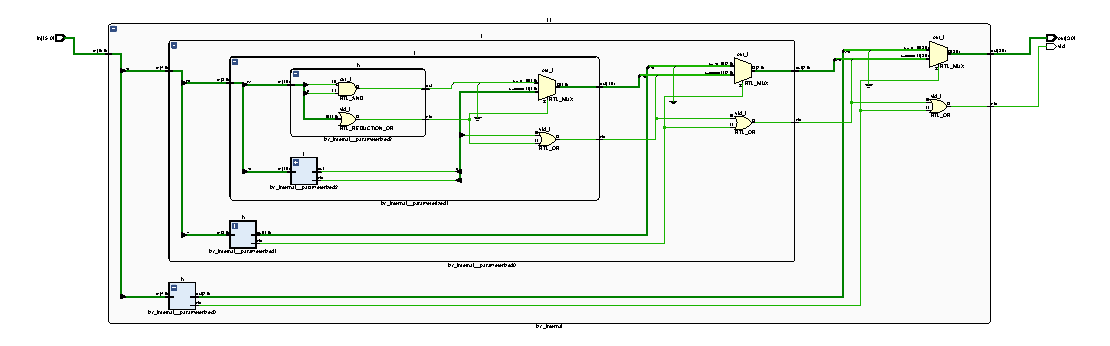
\includegraphics[width=1.3\textwidth]{figures/lzc_pacogen_vivado.pdf}
    }
    \caption{\cite{PACoGen}'s 16-bits LZC generated schematic}
    \label{fig:lzc_synthesized}
\end{figure}







\begin{figure}
    \centering
        \centering
        \includegraphics[width=\textwidth]{figures/core_op.drawio.pdf}
        \caption{\textit{Core op} schematic (conceptual)}
        \label{fig:core_op_ppu_schematic}
\end{figure}   


\begin{figure}
        \centering
        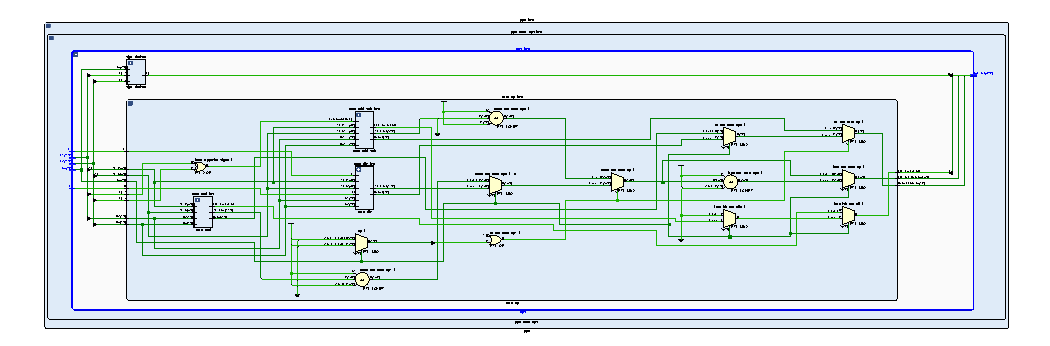
\includegraphics[width=\textwidth]{figures/core_op.vivado.pdf}
        \caption{\textit{Core op} schematic (Vivado)}
        \label{fig:core_op_ppu_schematic_vivado}
\end{figure}   




\subsection{Computation}


The computation stage implements the modules described in Section \ref{Computation}.
The input operands are passed as FIR types and the operation is selected by the \textit{op} (short for \textit{operation}) signal.
First, the FIR signal is unpacked in its 3 components (sign, total exponent, and fraction), and the latter two are routed into the submodules. The signs are instead routed into the \textit{sign decisor} module. The involvement of the sign components in the core operations is minimal, as they only indirectly affects the \textit{add / subtract} module which needs the information about whether the signs are even, and some bit-alignments before outputting the newly computed \textit{te} and \textit{frac}.




\subsubsection{Adder/Subtractor}

The adder/subtractor implements the set of operations described in section \ref{sec:posit_ops}. The majority of the steps required for either operation is shared, hence the reason why a common module.
As a consequence of the preliminary \textit{pre-condition} step described in section \ref{sec:posit_extraction}, there is here no need to perform any operation to determine the final sign: the first operand is the largest in magnitude, therefore its sign will determine the output's as well. This consideration saves quite some logic.

The fractions are shifted upwards by a safe\footnote{\texttt{MAX\_TE\_DIFF}: size such that, if the second operand fraction had to be downshifted by the largest total exponent difference, no bits would be lost} constant amount and the second operand fraction is downshifted back by the difference of the total exponents, such that their \textit{effective exponent} is even and fractions are weighted equally.
Next, the fractions are added/subtracted together -- depending on the \textit{have opposite sign} flag -- before being routed into the \textit{core add} and \textit{core sub} sub-modules. Those implement the steps that differ between the two: the addition module needs to detect whether fraction overflow ($f \ge 2.0$) has occurred\footnote{recall from section that $(1.f_1) + [(1.f_2) \cdot 2^{-b}] \in [1.0, 4.0) \equiv [1.0, 3.999\dots]$, i.e. the integer part of the resulting fraction will, at most, occupy $\lceil\log_2(3)\rceil = 2$ bits} and fix that; the subtraction module needs to do the symmetrical operation, i.e. detect fraction underflow ($f < 1.0$) and fix that.

Fixing an overflow is straightforward: the fraction is downshifted by $1$, in order to obtain the canonical fraction format again, and the exponent is matched via an increment\footnote{e.g.: $10.010 \cdot 2^{\epsilon} \equiv (1.001 \cdot 2^1) \cdot 2^{\epsilon} \equiv 1.001 \cdot 2^{\epsilon + 1}$}. Shifting the fraction down however, is not a carefree operation: the least significant bit can be a $1$ and information about whether a truncation occurred must be preserved and forward-propagated in order to get the subsequent rounding right.

Fixing an underflow is not as straightforward as fixing an overflow:
the resulting fraction\footnote{$(1.f_1) - [(1.f_2) \cdot 2^{-b}] \in [0.0, 2.0) \equiv [0.0, 1.999\dots]$} can span from
% $0$ to $1.999\dots$ -- i.e.
$(1.f) \cdot 2^{-\infty}$ to $(1.f) \cdot 2^{0}$; this means that an arbitrary number of zeros can precede the $1$ that will constitute the most significant bit of a fraction.
This is the ideal place where a LZC finds employment, and where the second instance of the LZC presented in Figure \ref{fig:lzc_synthesized} will be used.
The figure returned by the LZC module will be used to (dynamically) shift the resulting fraction back in its canonical representation, and simultaneously update the total exponent difference.

The parent module -- \textit{core add/sub} -- will finally select, via the \textit{have same sign} flag, the appropriate resulting (total exponent, fraction) pair, and route them off the module, together with the \textit{is truncated} flag for later correct rounding computation.

\begin{figure}
    \centering
    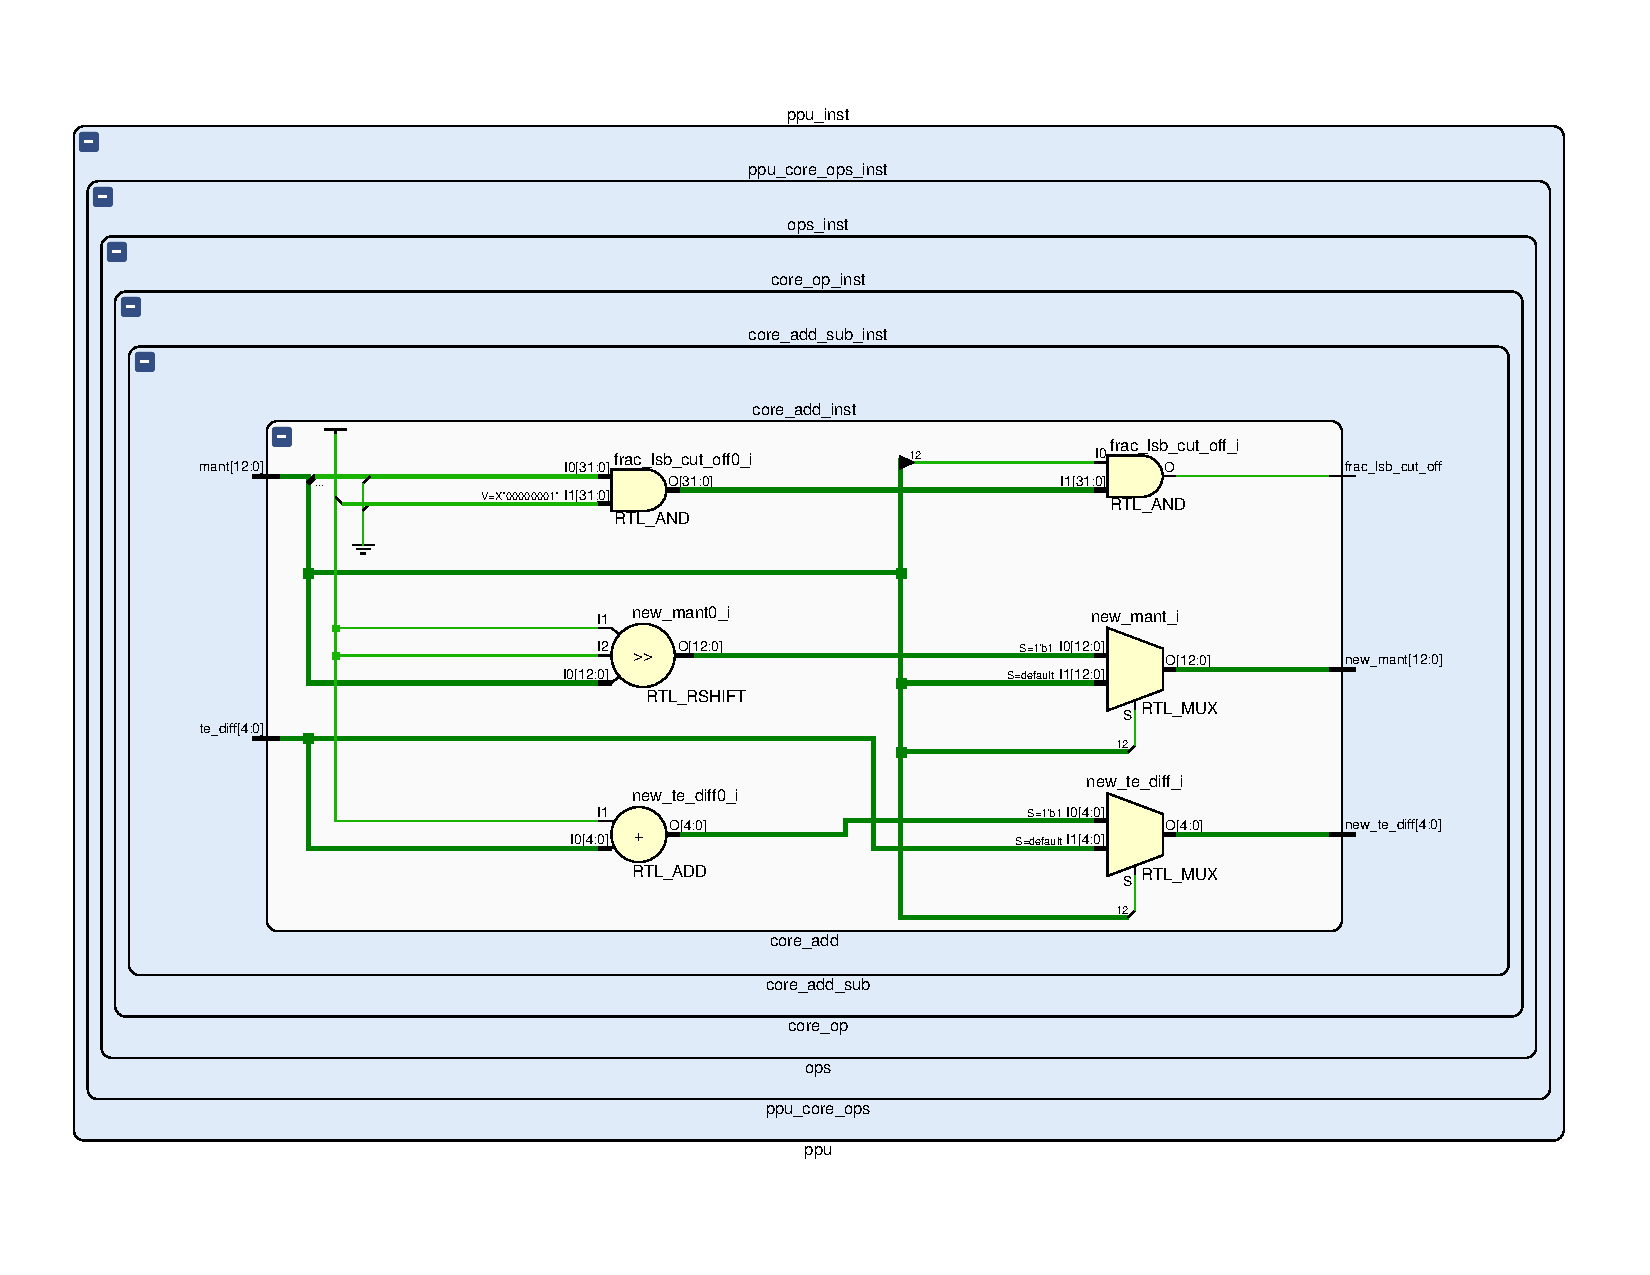
\includegraphics[width=\textwidth]{figures/core_add_vivado.pdf}
    \caption{\textit{Core add} (Vivado)}
    \label{fig:core_add_vivado}
\end{figure}%
\begin{figure}
    \centering
    \includegraphics[width=\textwidth]{figures/add-sub-core.drawio.pdf}
    \caption{\textit{Core add/sub} (conceptual)}
    \label{fig:core_add_sub_schematic_conc}
\end{figure}%

\begin{figure}
    \centering
    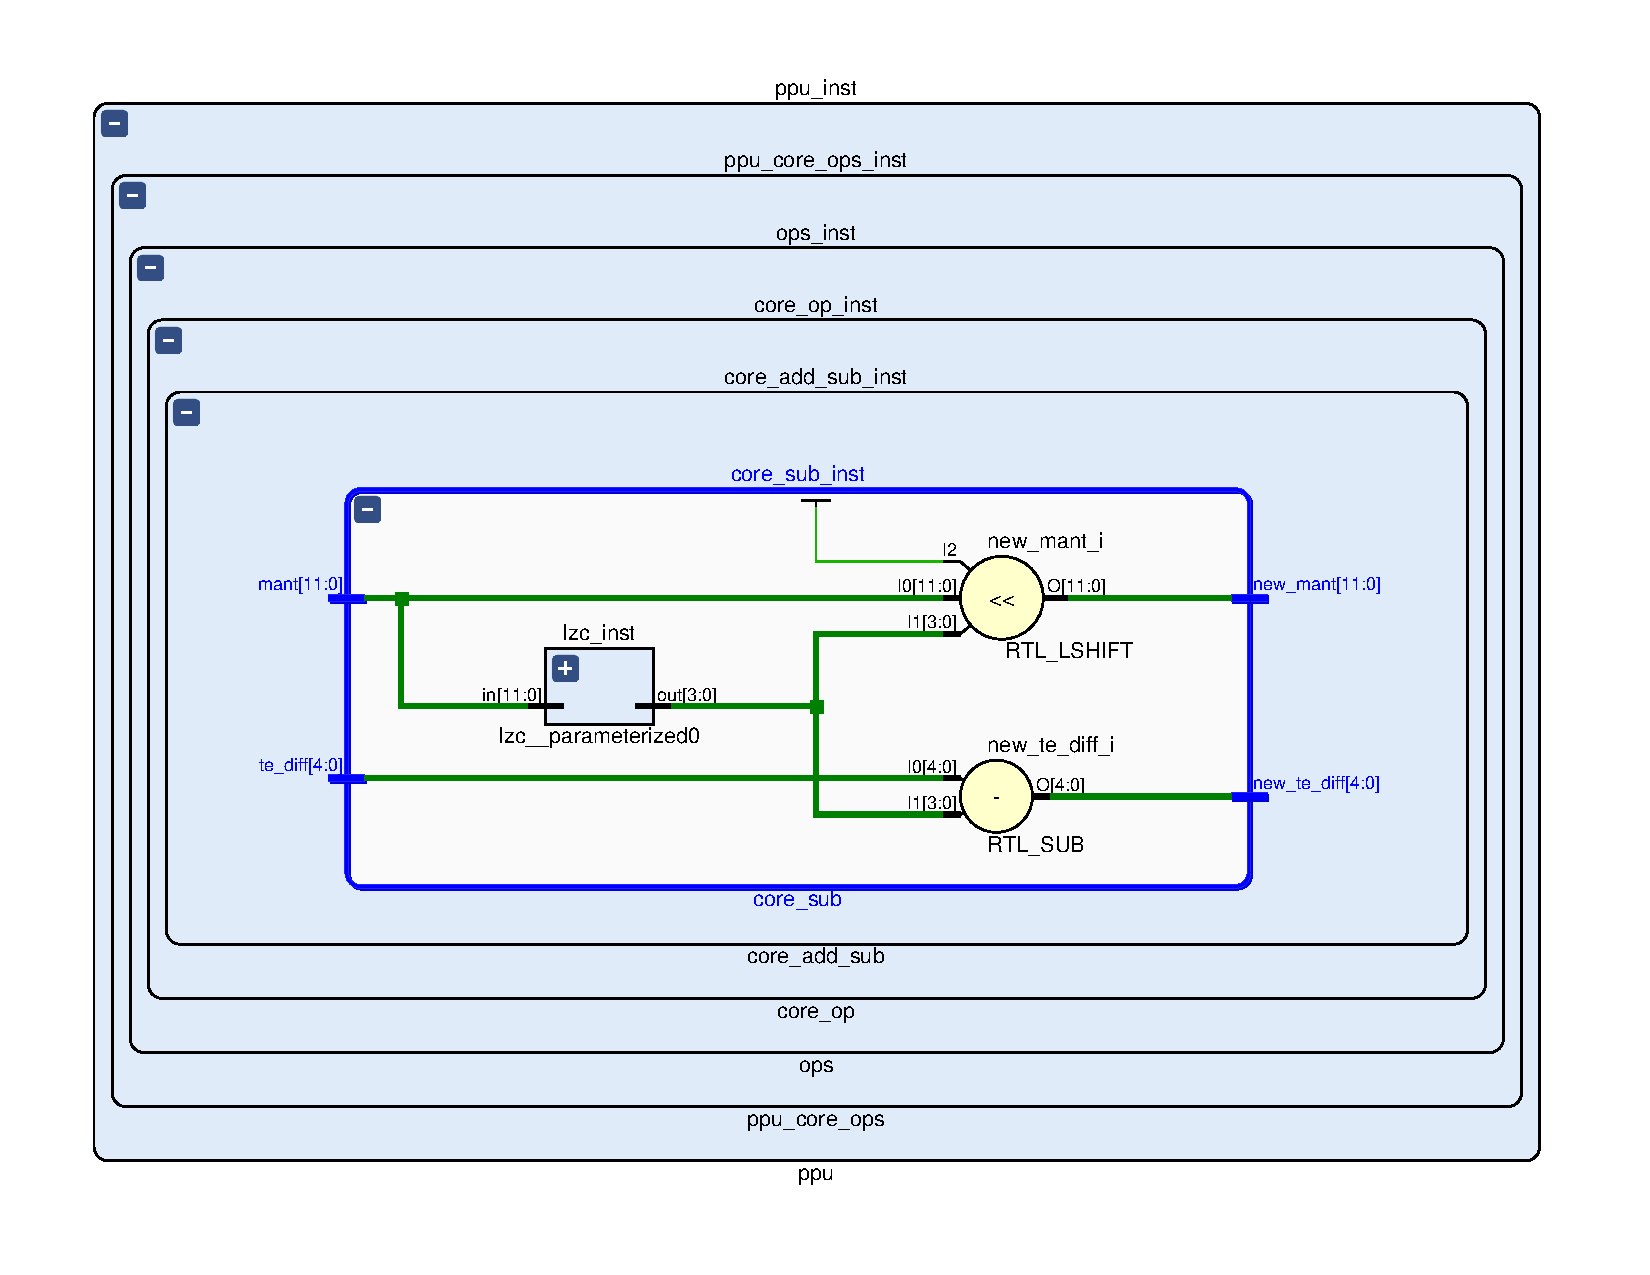
\includegraphics[width=1\textwidth]{figures/core_sub_vivado.pdf}
    \caption{\textit{Core sub} (Vivado)}
    \label{fig:core_sub_vivado}
\end{figure}

\begin{figure}
    \centering
    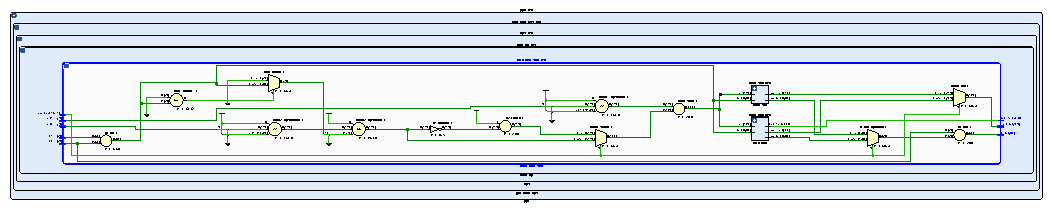
\includegraphics[width=1\textwidth]{figures/core_add_sub_vivado.pdf}
    \caption{\textit{Core add/sub} (Vivado)}
    \label{fig:core_add_sub_vivado}
\end{figure}%




\subsubsection{Multiplier}

\begin{figure}
    \centering
    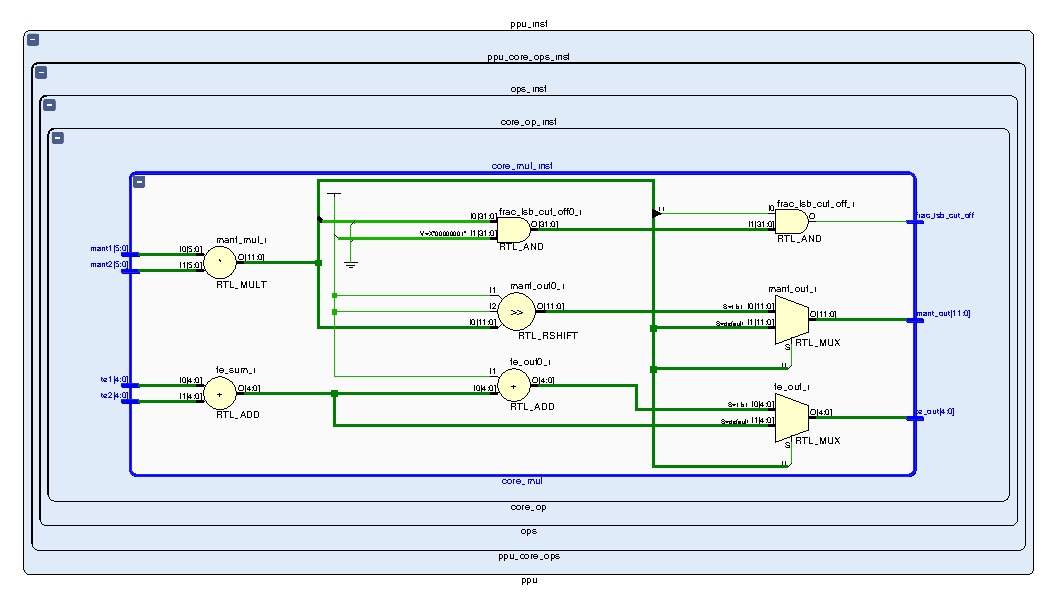
\includegraphics[width=\textwidth]{figures/mul_vivado.pdf}
    \caption{\textit{Core multiplier schematic} (Vivado)}
    \label{fig:mul_vivado}
\end{figure}


The multiplier computes the product of the fractional components of the two operands and sums their total exponents (\textit{te}). Similarly to the addition fraction overflow can occur: if it does indeed occur, a flag \textit{is truncated} is asserted to notify whether the least significant bit is a $1$, the fraction is shifted back by 1 unit to restore the canonical fractional representation and the total exponent is incremented by 1 to make up for the downshift.

The unsigned integer multiplier present in the schematic is inferred by the synthesys tool. 
% \hl{check}
%





\subsubsection{Divider}\label{divider_hardware_ppu}

% \hl{reformulate if time allows}

The core divider unit encompasses the implementation of the steps described in section \ref{Approximated_Algorithms}.

First, an approximation of the reciprocate of the second operand mantissa is computed using algorithm \ref{alg:reciprocal_approx_modified_drom} adapted to fixed-point unsigned integer arithmetic.
Next, that output is fed into the Newton Raphson stage.
Note however, that this unit as is, comes at an expensive cost, resource-wise, compared to a lighter but slower hypothetical implementation of a Newton Raphson divider.

With reference to an 8-bit posit division operation, the core divider instance is inferred as figure \ref{fig:div2vivado}. As mentioned throughout the this manuscript, this core is ``synthesis-time" configurable:
this investment is paid off in terms of results accuracy obtained, as reported later in table \ref{table:comparison_div_against_pacogen_table}.

    \begin{figure}
        \includegraphics[width=1\textwidth]{figures/newton_raphson_drawing.drawio.pdf}
        \caption{\textit{Core div} (conceptual)}
        \label{fig:nr_schematic}
    \end{figure}

    \begin{figure}
        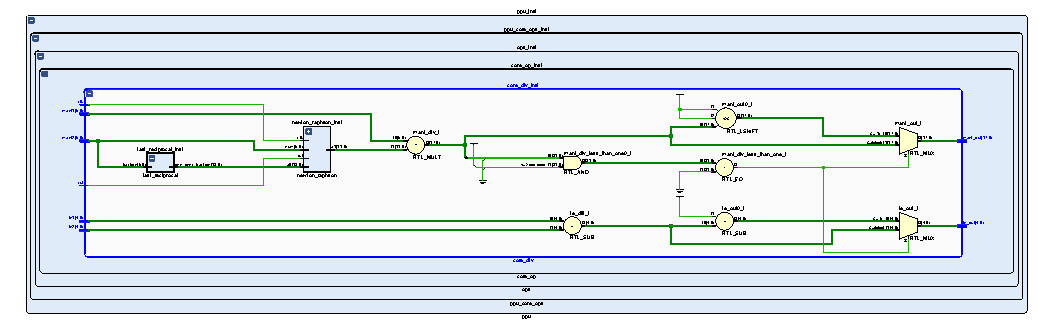
\includegraphics[width=1\textwidth]{figures/div_vivado.pdf}
        \caption{\textit{Core div} (Vivado)}
        \label{fig:div1vivado}
    \end{figure}
    \begin{figure}
        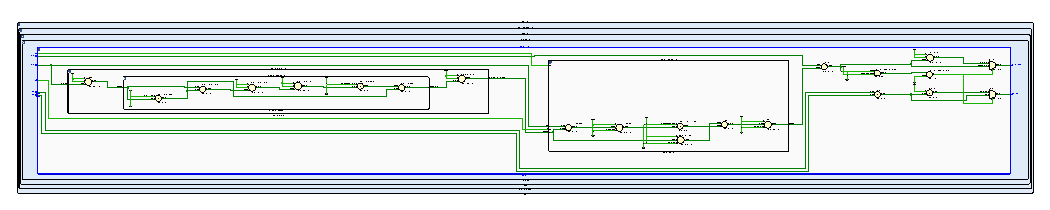
\includegraphics[width=1\textwidth]{figures/div_opened_vivado.pdf}
        \caption{\textit{Core div} opened (Vivado)}
        \label{fig:div2vivado}
    \end{figure}








\subsection{Normalization}

The \textit{normalization} stage performs the reverse operation of the \textit{extraction} stage; indeed it rebuilds the posit from the fields output by the computation stage.



\begin{figure}[h!]
    \begin{center}
    \includegraphics[width=1\textwidth]{figures/fir-to-posit-drawing.drawio.pdf}
    \caption{FIR to Posit}
    \label{fig:fir2posit_ppu}
    \end{center}
\end{figure}

A FIR is fed as input to the normalization unit, also referred to as ``FIR-to-Posit".
The FIR is unpacked in its sign (\texttt{sign}), exponent (\texttt{total\_exp}), and fraction (\texttt{frac\_full}) fields.
\texttt{frac\_full} represent the full fraction, formatted as a \texttt{Fx<0, \_>} fixed-point, without any truncation being applied from the previous (computation) stage.

Within ``pack fields" the total exponent is separated into $k$ (regime value) and $e$ (exponent value). Hardware-wise this is a simple couple of shifts: \texttt{k = total\_exp >> ES}, \texttt{exp = total\_exp - (k << ES)}, that corresponds to form and remainder of the division.
The value of $k$ establishes the regime size and, in turn, the remaining fields, including the size of the final fraction. 
The fraction, combined with its final length determines the value of the rounding bits (G, R, S) as brought to the attention in figure \ref{fig:fraction_before_rounding}.

``Posit encoder" stitches together the fields into one bit-string, which is the un-rounded posit.
Then, \textit{nearest-even} rounding is applied: this is a simple bit increment on posit based on the logic value of the other input flags.

Lastly, the sign is set: this consists of either no intervention if the resulting posit is meat to represent a positive value (sign = 0), or bit-string two's complement otherwise (sign = 1).



\subsection{Conversions}

% \hl{insert fig simil clarinet}






\begin{figure}
        \centering
        \includegraphics[width=1\textwidth]{figures/top_no_conversions.pdf}
        \caption{\textit{bare} PPU}
\end{figure}
\begin{figure}
        \includegraphics[width=1\textwidth]{figures/top_P2F.pdf}
        \caption{\textit{bare} PPU with support to posit-to-float conversion}
        \label{fig:top_p2f_00000001}
\end{figure}
\begin{figure}
        \includegraphics[width=1\textwidth]{figures/top_all.pdf}
        \caption{\textit{bare} PPU with support to posit-to-float and float-to-posit conversions}
\end{figure}



\begin{figure}
    \centering
    \includegraphics[width=\textwidth]{figures/posit_to_float_and_float_to_posit.pdf}
    \caption{Posit to Float and Float to Posit}
    \label{fig:posittofloatandfloattoposit}
\end{figure}

\begin{table}
\begin{center}
\begin{tabular}{||c c c | c||}
    \hline
    op & $in_1$ & $in_2$ & $out$ \\ [0.5ex]
    \hline\hline
    \texttt{+} & $p_1$ & $p_2$ & $p_1 + p_2$ \\
    \hline
    \texttt{-} & $p_1$ & $p_2$ & $p_1 - p_2$ \\
    \hline
    \texttt{*} & $p_1$ & $p_2$ & $p_1 * p_2$ \\
    \hline
    \texttt{/} & $p_1$ & $p_2$ & $p_1 / p_2$ \\
    \hline
    \texttt{f2p} & $f$ & $-$ & \texttt{f2p}$(f)$ \\
    \hline
    \texttt{p2f} & $-$ & $p$ & \texttt{p2f}$(p)$ \\
    \hline
\end{tabular}
\captionof{table}{PPU operations. $+,\ -,\ \times,\ \div,$ \texttt{f2p}, \texttt{p2f} encoded progressively from \texttt{0b000} to \texttt{0b101}.}
\label{Tab:table_ops_ppu}
\end{center}
\end{table}





\section{Pipelined architecture}\label{pipelined_ppu_section}


The first iteration of the design presented in the previous Section was based on a single stage data-path.


\begin{figure}
    \centering
    \includegraphics[width=1\textwidth]{figures/pipeline_drawio1.pdf}
\end{figure}
\begin{figure}
    \includegraphics[width=1\textwidth]{figures/pipeline_drawio2.pdf}
    \caption{Non-pipelined vs pipelined circuit} 
    \label{fig:pipeline_vs_nonpipeline}
\end{figure}

Pipeline-ing is a common technique adopted in digital design and computer architecture to speed-up\footnote{this can mean different things in different contexts: here we refer at higher output rate} the operations, by decomposing a long combinatory chain with a delay of $t_{pd_0}$ into $N$ shorter combinatory paths having different delays $t_{pd_1}, \dots t_{pd_{N}}$, each one smaller than $t_{pd_0}$; this can loose the requirements on the \textit{setup} and \textit{hold} times of the registers so that the overall circuit can operate at higher clock speed. The throughput, defined as the time between two different $d_{out}$ presented on the output, goes from $1/clk_1$ to $1/clk_2$, thus increases according to what has been stated.
        The latency, on the other hand, defined as the time it takes to a given input to traverse the sequence and turn up on the output, alters from $1/clk_1$ to $N \cdot (1/clk_2)$, which may be larger or smaller than the initial one

With reference to figure \ref{fig:pipeline_vs_nonpipeline}, the \textit{speedup} is defined as\footnote{\cite{lilja_pipelining_2004} $speedup = T_{non-pipelined}/T_{pipelined}$} equation \ref{equ:speedup_equation2},
        \begin{equation}\label{equ:speedup_equation2}
            \begin{aligned}
                speedup &= \frac{1/f_{clk_1}}{1/f_{clk_2}} \\
                &= \frac{f_{clk_2}}{f_{clk_1}} = \\
                &= \dfrac{\dfrac{1}{t_{cq} + t_{su} + \max\{t_{pd_1}, \dots, t_{pd_N} \}}}{\dfrac{1}{t_{cq} + t_{su} + t_{pd_0}}} = \\
                &= \frac{t_{cq} + t_{su} + t_{pd_0}}{t_{cq} + t_{su} + \max\{t_{pd_1}, \dots, t_{pd_N} \}}
            \end{aligned}
        \end{equation}
    %
        \begin{figure}
            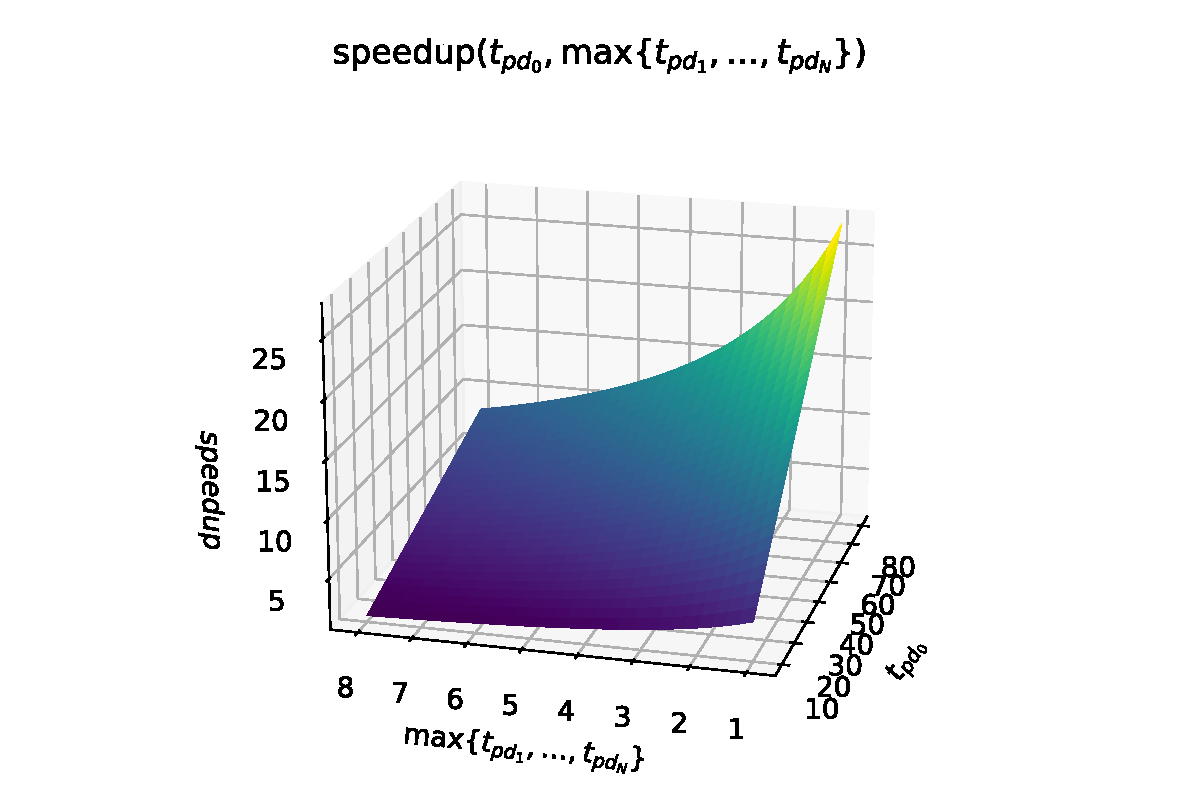
\includegraphics[width=1\textwidth]{figures/3d_plot_speedup.pdf}
            \captionof{figure}{Pipelining speedup}
            \label{fig:speedupplot}
        \end{figure}
where it assumes a hyperbolic shape with respect to the decreasing maximum new delay, ever more emphasized the higher the non-pipelined delay $t_{pd_0}$ is.\footnote{$t_{cq}$ (clock-to-q delay) and $t_{su}$ (setup time) are technology-dependent parameters}

The first design iteration of the pipelined PPU breaks the combinatory path between each top level stage: one registers pipe will be interposed between the \textit{extraction} and \textit{operations} stages, and the other between \textit{operations} and \textit{normalization} stage (figure \ref{fig:top_p2f_00000001}  $\rightarrow$ \ref{fig:top_all_PL2}).

The second provisional iteration adds a pipe of registers within the \textit{computation} module -- specifically, the core divider: this is meant to break the critical path, part of the divider instance. This bottleneck was very expected since the \textit{fast reciprocate} + \textit{Netwon Raphson} steps are largerly more resources intensive than the other three operations.

The design as described however, cannot function as is: we have introduced an additional pipeline stage that only affects a subset of the whole unit and conflicting data would arise if not orchestrated by a purposefully arranged control unit.



\begin{figure}
    \centering
    \includegraphics[width=\textwidth]{figures/pipeline_ops_diagram1.pdf}
    \caption{Timing diagram of posit operations without pipelining}
    \label{fig:timing_diagram_4_stagesdiv_3stagesothers_without_pipelining}
\end{figure}
\begin{figure}
    \centering
    \includegraphics[width=\textwidth]{figures/pipeline_ops_diagram2.pdf}
    \caption{Timing diagram of posit operations with pipelining}
    \label{fig:timing_diagram_4_stagesdiv_3stagesothers_with_pipelining}
\end{figure}



The timing diagram in figure \ref{fig:timing_diagram_4_stagesdiv_3stagesothers_with_pipelining}  visually reveal the meaning of the previous sentence: each \textit{non-div} operations goes through the three \textit{execution}-\textit{computation}-\textit{normalization} (E-C-N) stages, whereas \textit{div} is broken down in two sub-stages (C1, C2) within the \textit{computation} phase (figure \ref{fig:ppu_with control_unit1}).

It becomes evident that each time a transition \textit{non-div} $\rightarrow$ \textit{div} operation requires to invalidate the output for one cycle: this comes from \textit{div} taking one cycle longer to reach the normalization stage; the output is garbage until the \textit{div}'s N-stage is complete. The red cross in the diagram signifies that the output is not valid in the corresponding cycle

On the other hand, a transition \textit{div} $\rightarrow$ \textit{non-div} operation requires the \textit{non-div} operation to stall its execution. E and C would be able to run concurrently, however the normalization stage would conflict with the previous operation. Stalling the execution -- anytime before the conflict -- is the conventional way to go around this.

These asymmetries introduced to not slow down (i.e. increase latency) the whole unit when fed with \textit{non-div} operations is paid with the need of a proper control unit running a finite state machine able to detect \textit{div}-\textit{non-div} (and vice-versa) transitions, emitting \textit{stall} and \textit{valid-output} signals to the core PPU and output respectively.


This approach hinders another significant implication: the finite state machine can only stay \textit{locked} on the operation so long as low \textit{div} $\rightarrow$ \textit{non-div} operation hopping occurs. Conversely, the finite state machine would lose track, and the only solution would be at a different layer of the stack.
This can be worked out by modifying the compiler to interpose a \texttt{nop} instruction every time a \textit{div} $\rightarrow$ \textit{non-div} transition occurs, effectively mimicking a stall event.



To mitigate this circumstance two solutions are in sight: the first one being a compiler modification. This may not be the easy solution, and involves intercepting the transitions \textit{div} $\rightarrow$ \textit{non-div} and interpose a \texttt{nop} instruction.

The second solution, the easier one, consisting in slowing down the rest of the chain to the same number of cycle the longest operation take. This is by no means a clever choice, but can still be considered acceptable under some circumstances.




\begin{figure}
\centering
    \includegraphics[width=1\textwidth]{figures/top_all_PL2.pdf}
    \caption{3-stage pipelined PPU}
    \label{fig:top_all_PL2}
\end{figure}
\begin{figure}
\centering
    \includegraphics[width=1\textwidth]{figures/top_all_PL3.pdf}
    \caption{4-stage pipelined PPU}
    \label{fig:top_all_PL3}
\end{figure}


\begin{figure}[h!]
    \centering
    \includegraphics[width=1\textwidth]{figures/ppu_all_with_control_unit_3a.pdf}
    \caption{4-stage div, 3-stage add/sub/mul. Control unit issues \textit{stall} signals to the core PPU}
    \label{fig:ppu_with_control_unit1}
\end{figure}%
 
\begin{figure}
    \centering
    \includegraphics[width=1\textwidth]{figures/ppu_all_with_control_unit_3b.pdf}
        \caption{4-stage operations. Control unit only asserts \textit{valid\_out}}
        \label{fig:ppu_with_control_unit2}
\end{figure}%

\begin{figure}
    \centering
    \includegraphics[width=1\textwidth]{figures/simple_fsm.pdf}
    \caption{Simple Finite State Machine}
    \label{fig:simple_fsm}
\end{figure}



Charts in Figures \ref{fig:spartan7_stages_vs_freqlatency_64_32_8_2} and \ref{fig:spartan7_stages_vs_freqlatency_64_64_16_2} show the progression of highest frequency/lowest latency achievable as the number of pipeline stages increases\footnote{specifically, moves from no pipeline to 3 and 4 stages, as described}, on a Spartan7 \texttt{xa7s6cpga196-2I} FPGA device, in two different configurations: figure \ref{fig:spartan7_stages_vs_freqlatency_64_32_8_2} is referred to a  PPU core supporting $P\langle8,2\rangle$ posits + conversions to single-precision floating point, figure \ref{fig:spartan7_stages_vs_freqlatency_64_64_16_2} is referred to a PPU core supporting $P\langle16,2\rangle$ posits + conversions to double-precision floating point.
As expected, in both cases the maximum frequency grows with the number of stages ($\sim \mathcal{O}(\log(n))$) -- as the delay of progressively shorter paths decreases.

The latency\footnote{$\#\ \text{stages} \cdot 1/f$} though, has not a-priori defined behavior.
In both cases, it's interesting to look at the alteration between 2 and 3 stages: the advantage over the maximum frequency gain is, respectively, marginal and insignificant at best, meaning that in those case it is probably wasteful the addition of the third, mid \textit{operation} registers pipe.





\begin{figure}
        \centering
        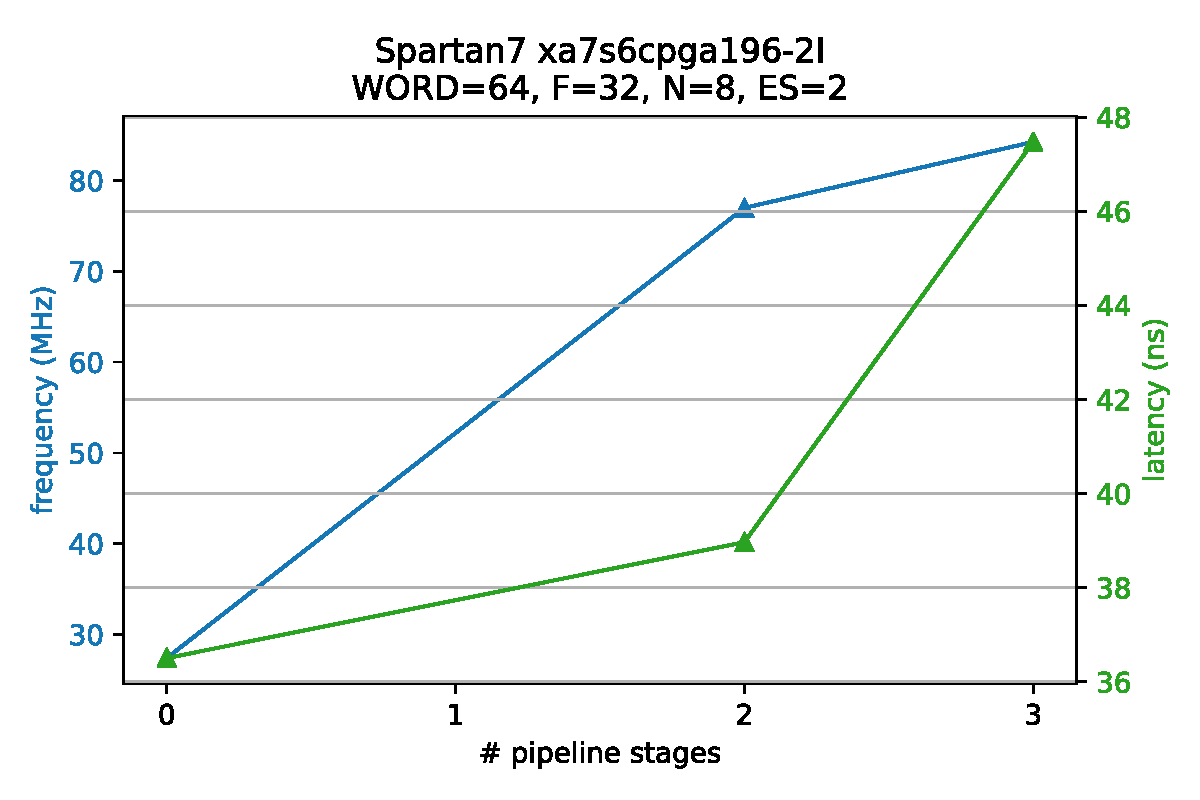
\includegraphics[width=1\textwidth]{figures/Spartan7_xa7s6cpga196-2I_64_32_8_2_freq_lat.pdf}
        \caption{\posit{8}{2} pipeline stages impact on frequency and latency}
        \label{fig:spartan7_stages_vs_freqlatency_64_32_8_2}
\end{figure}
\begin{figure}
    \centering
    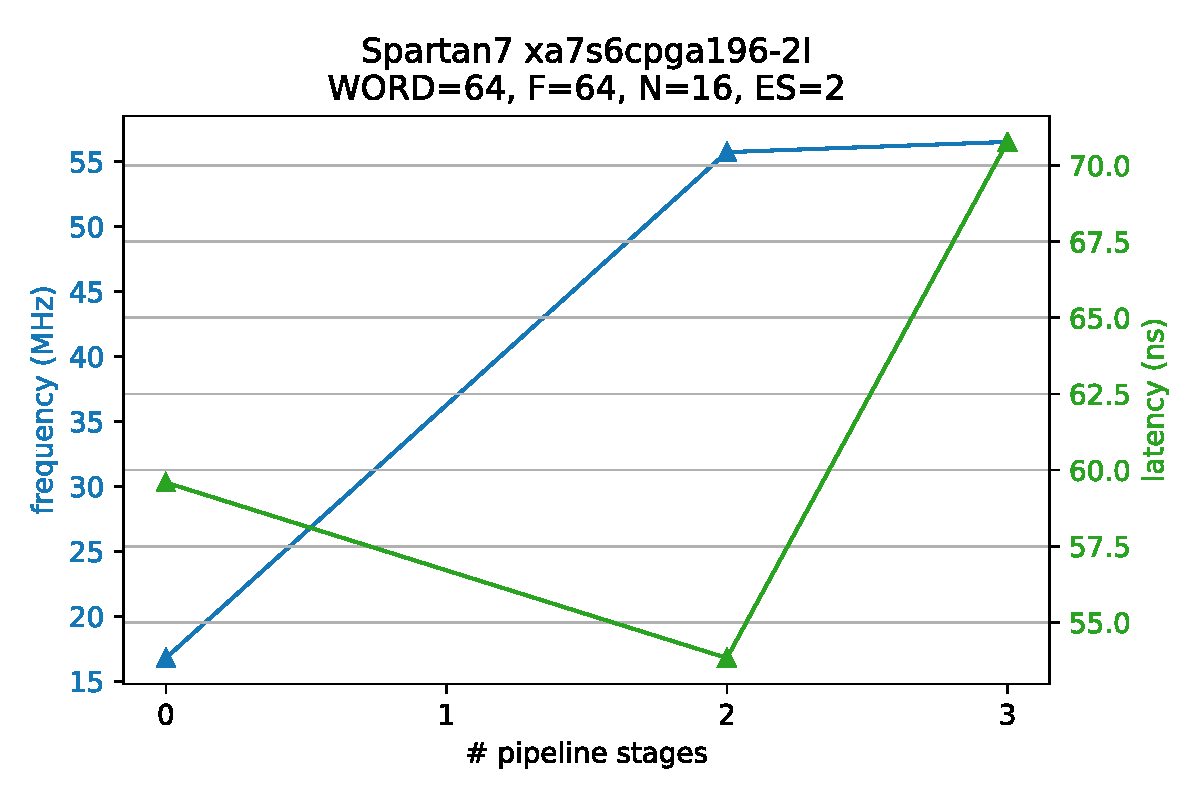
\includegraphics[width=1\textwidth]{figures/Spartan7_xa7s6cpga196-2I_64_64_16_2_freq_lat.pdf}
    \caption{\posit{16}{2} pipeline stages impact on frequency and latency}
    \label{fig:spartan7_stages_vs_freqlatency_64_64_16_2}
\end{figure}




\section{Synthesis and characterization}

\subsection{Power}
Static power is constant regardless of the circuit's current operating state, which consists of leakage currents from supply to ground via the transistors. This phenomenon is due to the non-idealities of the transistors. 

Dynamic power is the power consumed by transistors when they are switching. 
This power contribution is mainly due to the charging of capacitive loads connected to the transistor (i.e. gates of adjecent transistors, wires parasitic capacitances, et cetera). 
Some fraction of dynamic power is consumed during the state transition, when high and low side of the transistors are partially open, creating a direct path from suppy voltage to ground. The latter however, is relatively irrelevant compared to the capacitance charging, thus it is often neglected.

The total power consumption of a circuit can be modeled as:
\begin{equation}\label{equ:power_cmos_equation}
P_{tot} = \underbrace{V_{CC} \cdot I_{leak}}_{P_{static}} + \underbrace{\alpha \cdot C \cdot V_{CC}^2 \cdot f}_{P_{dynamic}}
\end{equation}

where $V_{CC}$ is the supply voltage, $I_{leak}$ is the total leakage current, $\alpha$ is the activity factor, $C$ is the driven capacitance and $f$ is the operating clock frequency of the circuit.

From (\ref{equ:power_cmos_equation}) the knobs one can act on to reduce the power consumptio are:
\begin{itemize}
\item lowering the operating voltage (if applicable),
\item cut-off unnecessary toggling,
\item adopting clock gating techniques. This shuts down the non currently active subsystems, effectively bringing the activity factor $\alpha$ down to zero.
\end{itemize}




\subsection{Timing}
One important parameter that affects how fast a design can run is the critical path - the longest path a signal must travel between two endpoints before the next clock edge. 
The maximum speed\footnote{speed and clock frequency are used interchangeably} is determined by slack, that is, the time leeway before the deadline.
Positive slack means all signals arrive on time, and there is room for improvements in terms of clock frequency. Negative slack means that the circuit has a timing issue and will not operate properly at the given clock frequency.
In that case the designer must either resort to shortening the critical path, or acknowledge that the circuit will not operate at a the desired clock rate.

\subsection{Synthesis}

Once the device was validated, its gate-level description was obtained by resorting to a commercial logic synthesis tool, Xilinx Vivado\footnote{Linux's 2020.2.2 version}.

% After passing all the behavioral simulation tests, a lot of different, meaningful, configurations of the posit processing unit have been generated and synthesized.


% --------------------------------------------------------


The basic logic element in the
% Series 7
FPGAs by Xilinx is the Configurable Logic Block (CLB). Each CLB contains
% two
slices and is connected to the interconnection matrix via a dedicated switch. Slices are the fundamental resource and most importantly include Look Up Tables (LUTs) and registers. The former can be used to implement combinational logic and, combined with the latter, form a sequential resource. Additionally, multiplexers are embedded within slices to route internal signals.
Special resources, known as digital signal processing slices are high-speed blocks which include, among others, circuitry for multiplication.


% --------------------------------------------------------




Due to the nature of a PPU, which is meant to be tightly integrated inside a broader system, that is, a host CPU, the following will follow the Out Of Context (OOC) design flow.
Synthesizing or implementing a module out of context requires that the tools be run in an ``out-of-context" mode\footnote{\url{https://docs.xilinx.com/r/2021.2-English/ug905-vivado-hierarchical-design/Out-of-Context-Commands}}.

Out Of Context synthesis (also known as bottom-up synthesis) refers to a synthesis flow in which each module has its own synthesis run. This generally involves turning off automatic IO buffer insertion.

The OOC design flow entails the following:
\begin{itemize}
\item external signals are not routed to the IO pins of the chip. This means that interfacing signals\footnote{those providing inputs and outputs to the PPU module, i.e. the two operands, the operator selector and the resulting output} do not need to stretch through the entire chip
\item and consequently wires are shorter, delays are reduced and higher frequency rates can be achieved;
\item moreover the capacitive load of the IO pins is removed from the equation allowing for a even higher frequency rate.
\end{itemize}




The synthesis reports originated from the tool, run on three different Xilinx FPGA families -- Spartan7, Kintex7, and Virtex UltraScale+ -- parametrized by posit/float datatype formats, are reported in Tables (in Appendix) \ref{table:table_xa7s6cpga196-2I}, \ref{table:table_xc7k325tffg900-2}, \ref{table:table_xcku060-ffva1156-3-e} and \ref{table:table_xcvu23p-fsvj1760-3-e} respectively.


The reason behind these three families, or rather those devices specifically, have been chosen as ``benchmark" comes from their characteristics: the Spartan7 and Virtex UltraScale+ sit on the opposite end of the spectrum of the entire Xilinx catalog -- the latter being on the top end. The Kintex7, on the other hand, while being a high-performace product, is the device installed on the popular Digilent Genesys 2 development platform.


Tables \ref{table:table_xa7s6cpga196-2I}, \ref{table:table_xc7k325tffg900-2}, \ref{table:table_xcvu23p-fsvj1760-3-e}, \ref{table:table_xcku060-ffva1156-3-e} bring light to the following facts:
\begin{itemize}
    \item the fastest speed can be reached on the Virtex UltraScale+ which -- everything elese being equal\footnote{e.g. (WORD, F, N, ES) = (64, 0, 8, 0)} -- is able to operate at $75 \%$ and $126 \%$ higher clock rate\footnote{highest clock rate defined as the reciprocate of the smallest clock period which, in turn, is defined as the clock period (T) minus the Worst Negative Slack (WNS). WNS being the margin between the current clock period and the smallest clock period the design could operate at, without violating the setup time} than the Kintex7 and Spartan7 respectively. This is an direct consequence of the fabrication technologies of those chips: 16\footnote{Virtex\textregistered UltraScale+\textsuperscript{TM} \url{https://www.xilinx.com/products/silicon-devices/fpga/virtex-ultrascale-plus.html}} vs 28\footnote{Kintex\textregistered-7 \url{https://www.xilinx.com/products/silicon-devices/fpga/kintex-7.html}} vs 28\footnote{Spartan\textregistered-7 \url{https://www.xilinx.com/products/silicon-devices/fpga/spartan-7.html}} nanometers.
    \item longer posit formats run at slower speed due to the growing (mostly) divider path length,
    %\item larger power is consumed on larger devices -- predominanly \textit{static},
    \item larger power is consumed at higher clock rate -- predominanly \textit{dynamic},
    \item the larger percentage of power consumed on the larger devices is the static component: this comes from keeping the chip powered on, and is not direcly related to the actual power drained by the design.
\end{itemize}



\section{Comparison with PACoGEN}

In order to complement and back up the claims stated in section \ref{Approximated_Algorithms}, we choose one of the most common works in literature related to Posit core generators, to compare our own design against.
PACoGen \cite{PACoGen} is a scientific paper published in mid 2019 where the authors designed one of the first \textbf{p}osit \textbf{a}rithmetic \textbf{co}re \textbf{gen}erators (hence the acronym). The foremost reason why this was chosen as reference target, is that its HDL implementation was released as open-source\footnote{\url{https://github.com/manish-kj/PACoGen}} under the BSD 3-Clause License.


The source code presents itself as three compartmentalized folders, one for each supported binary operation, i.e. \textit{add}, \textit{mul}, \textit{div}, each of whom implemented in a single HDL description file -- leaving thus little room for code (and resources) reuse.

The promise of PACoGen is to generate cores supporting operations over \textit{any} posit format.

The implementations of the adder and multiplier are as straightforward as they can get, as they can always produce exact results.

 The division however, has room for compromises and original choices. The way they go around that is the ``approximated algorithm" route: a  LUT storing the $M$ most significant bits of the reciprocate of the fractions followed by $S$ Newton Raphson iterations (figure \ref{fig:pacoge_divider_architecture}), narrowing down the accuracy at the finest level desired. The number of Newton Raphson iterations being
    \begin{equation*}\label{equ:regime_k_equation}
        S = \begin{cases}
        0, &\text{ if } N \le 8 \\
        1, &\text{ if } 8 < N \leq 16 \\
        2, &\text{ if } 16 < N \le 32 \\
        \end{cases}
    \end{equation*}
    or, in general, $S = \lceil \log_2(N / 8) \rceil$.

\begin{figure}
    \centering
    \includegraphics[width=0.6\textwidth]{figures/div_pacogen_architecture.pdf}
    \caption{\cite{PACoGen}'s PACoGen divider architecture}
    \label{fig:pacoge_divider_architecture}
\end{figure}


PACoGen does not support out of the box the posit formats $P\langle\_, 0\rangle$, which is unfortunate since, together with $P\langle16, 1\rangle$ and $P\langle32, 2\rangle$, $P\langle8, 0\rangle$ was the standard $8$-bit posit type at the time this work was carried out\footnote{The posit standard was ratified on March 2, 2022 (\url{https://posithub.org/docs/posit_standard-2.pdf}), pinning the exponent size at $2$ for any posit size $N$}.

To work around the limitation of not being able to compare division results between $P\langle\_, 0\rangle$ posits, we forked the repository and retrofitted all three modules to support $ES = 0$ posits class.


The result of the comparison (using the setup shown in Figure \ref{comparison_against_pacogogen_dut}, generated by comparing the division module
for all the desired combinations of posit formats is reported in table \ref{table:comparison_div_against_pacogen_table}, where \textit{LUT\_IN} and \textit{LUT\_OUT} are the sizes of the LUT used to store the precomputed most significant bits of the reciprocate of $\text{mant}_2$, interpreted as \texttt{Fx<1, B>} as wholly described in section \ref{aot_reciprocal_lut_technique}; and \textit{NR} indicates the number of Newton Raphson iterations. These three parameters are hard-coded in the original version of PACoGen.
The ``wrong [\%]" columns reports the percentages of result that differ from the ground truth division between two posits: these are tested against our software library (and others, where applicable).
Recall that \textit{proposed}'s divider consists of one Newton Raphson iteration preceded by what has been referred to as \textit{fast reciprocate} (figure \ref{fig:reciprocal_unsigned_workflow}).


These inexactnesses involve, in almost $100 \%$ of the cases, the least significant bit, which is, for the large part, always a fraction bit. This means that these ``errors" are as meaningless as they can get, both for PACoGen and proposed.
The benefit brought by the proposed approach in terms of accuracy, up to 16-bits posit, are also crystal clear.


Figure \ref{fig:comparison_against_pacogogen_dut_waveforms} shows waveforms of the comparison between PACoGen and proposed: the last four traces indicate -- when non-zero -- that an inexact posit division verified. The density of the \textit{spikes} gives a qualitative indication of their inexactness. The traces suffixed with \textit{off by 1} indicate that only the least significant bit is off, which is \~ always. These qualitative indicators are quantified in table \ref{table:comparison_div_against_pacogen_table}.


\begin{figure}
        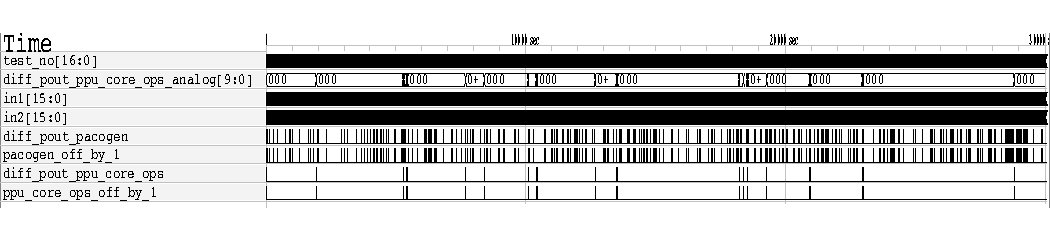
\includegraphics[width=\textwidth]{figures/waveform_div_against_pacogen.pdf}
        \caption{Waveform from the simulation of comparison between PACoGEN and the proposed unit}
        \label{fig:comparison_against_pacogogen_dut_waveforms}
\end{figure}




\begin{table}
\begin{center}
\begin{savenotes}
\begin{tabular}{ccccccccc}
    \toprule
     & & \multicolumn{4}{c}{PACoGen} & & \multicolumn{2}{c}{proposed} \\
    \cmidrule{3-6} \cmidrule{8-9}
    N & ES & LUT IN & LUT OUT & NR & wrong [\%] & & NR & wrong [\%] \\
    \midrule \midrule
    8 & 0 & 8 & 9 & 0 & 4.8 & & 1 & \textbf{1.4} \\
    8 & 1 & 8 & 9 & 0 & 5.4 & & 1 & \textbf{1.2} \\
    8 & 2 & 8 & 9 & 0 & 9.3 & & 1 & \textbf{2.1} \\
    8 & 3 & 8 & 9 & 0 & 13.5 & & 1 & \textbf{4.2} \\
    8 & 4 & 8 & 9 & 0 & 16.4 & & 1 & \textbf{7.5} \\
    \midrule
    16 & 0 & 8 & 9 & 1 & 10.0 & & 1 & \textbf{1.5} \\
    16 & 1 & 8 & 9 & 1 & 10.0 & & 1 & \textbf{0.6} \\
    16 & 2 & 8 & 9 & 1 & 8.8 & & 1 & \textbf{0.5} \\
    16 & 3 & 8 & 9 & 1 & 9.0 & & 1 & \textbf{0.1} \\
    \bottomrule
\end{tabular}
\end{savenotes}
\caption{Percentages of posits $P\langle N,ES\rangle$ inexact division results. \cite{PACoGen}'s PACoGen vs proposed}
\label{table:comparison_div_against_pacogen_table}
\end{center}
\end{table}


\begin{figure}
        \includegraphics[width=\textwidth]{figures/pacogen_vs_me_dut.pdf}
        \caption{Device setup for the comparison between PACoGEN Divider an the proposed one}
        \label{fig:comparison_against_pacogogen_dut}
\end{figure}